%!TEX root = ../thesis.tex
%*******************************************************************************
%****************************** Forth Chapter **********************************
%*******************************************************************************
\chapter{Experimentations , Results and Analysis}

% **************************** Define Graphics Path **************************
\ifpdf
    \graphicspath{{Chapter4/Figs/Raster/}{Chapter4/Figs/PDF/}{Chapter4/Figs/}}
\else
    \graphicspath{{Chapter4/Figs/Vector/}{Chapter4/Figs/}}
\fi

In this chapter, we will explain how data quality dimensions are implemented with Machine Learning (ML) techniques towards dirty datasets. 

\section{Experimental Methodology}  

The impact of the dirt data and data cleaning on ML in a dataset depends on a number of factors -- some factors depend on the data cleaning process, 

i.e., the error types to be cleaned and the cleaning methods; some factors depend on the ML
process, i.e., the model types used; and some factors depend on where the cleaning is performed during the ML process. Hence, in order to comprehensively investigate the impacts, we need to consider data cleaning an ML jointly in our experiments.

\section{The NettoyageML Schema}  

The NettoyageML relational schema consists of three relations as shown in Table ~\ref{table:nettoyage_ml} . Firstly will introduced the attributes of NettoyageML relational models, and then will explained 
the differences between these three relations.


\begin{itemize}
	\item {
		\textbf{Attributes for Dataset.} The first attribute is dataset, which is the input to the data cleaning and ML pipeline. Each dataset can have multiply types of errors and has an associated ML task. 
	}
\end{itemize}

\begin{table}[H]	
	\leftskip=3em
	\begin{flushleft}
		\leftskip=3em
		\textbf{R1 Vanilla}
	\end{flushleft}
	\begin{tabular}{|c|c|c|c|c|c|c|}
		\hline 
		Dataset & Error Type & Detection & Repair & ML Model & Scenario & Flag \\ 
		\hline 
	\end{tabular} \linebreak	

	\begin{flushleft}
		\leftskip=3em
		\textbf{R2 (With Model Section)}
	\end{flushleft}
	\begin{tabular}{|c|c|c|c|c|c|c|}
		\hline 
		Dataset & Error Type & Detection & Repair & Scenario & Flag \\ 
		\hline 
	\end{tabular} \linebreak

	\begin{flushleft}
		\leftskip=3em
		\textbf{R3 (With Model Selection and Cleaning Method Selection)}
	\end{flushleft}	

	\begin{tabular}{|c|c|c|c|c|c|c|}
		\hline 
		Dataset & Error Type & Scenario & Flag \\ 
		\hline 
	\end{tabular} \linebreak
	\caption{NettoyageML Relational Schema}
	\label{table:nettoyage_ml}
\end{table}

Even for one error type, they might appear in a dataset in various distributions and hence affect ML models in complicated ways. To study the impact of the real-world error types and distribution on ML models, we mostly use real-world-dataset with real errors, and we apply various cleaning methods to detect and repair the errors in them.


\begin{itemize}
	\item {
	\textbf{Attributes for Data Cleaning.}	
		The error type attribute describes
		which type of dirtiness we are testing. We consider five most
		common types of dirtiness that are considered in the ML and
		DB communities: missing values, outliers, duplicates, inconsistencies, and mislabels. For each error type, there exist multiple
		cleaning methods, and each cleaning method includes an error
		detection component and an error repair component.
	}
\item {
	\textbf{Attributes for ML.}	
	The ML model describes the algorithm of
	training and prediction. Different ML models may have different
	robustness or sensitivity to dirty data.
}
\item {
	\textbf{Flag Attribute.}	
	\textit{The flag attribute summarizes } the impact of data cleaning on ML of an experiment into three categories “\textbf{P (positive)}”, “\textbf{N (negative)}” 
	or “\textbf{S (insignificant)}”, indicating whether
	the cleaning has a positive, negative, or insignificant impact on
	the ML performance respectively.
}
\end{itemize}

Given these attributes, we designed three relations as shown Table ~\ref{table:nettoyage_ml}
\textit{R1} shows the vanilla of the a NettoyageML relation schema with the key 
\textit{ \{\ dataset, error type, detect, repair, ML model, scenario, flag \}\ }
Every tuple of \textit{R1} represents \underline{a hypothesis} or \underline{an experiment:}
how does cleaning some type of error using a detection method and a repair method affect a ML model for a given dataset?
We also consider other two versions of relations in NettoyageML. 

Compared with \textit{R1}, \textit{R2} eliminates the ML model attribute. In this case,
we try different models during training and select the model that
has the best validation accuracy (or F1 score) as the model to be
considered in an experiment in \textit{R2}. 

Every tuple of R2 represents a hypothesis or an experiment: how does cleaning some type of error using a detection method and a repair method affect the best
ML model for a given dataset? 

\textit{R3} further eliminates the cleaning method (detection and repair) attributes. In this case, in addition
to model selection, we also try different cleaning methods and select the cleaning method that results in the best validation accuracy as the cleaning method to be considered in an experiment in \textit{R3}.
Every tuple of \textit{R3} represents a hypothesis or an experiment: how
does the best cleaning method affect the predictive performance of
the best model for a given dataset?

All three relations can also be extended with other attributes that are associated with an experiment, which may help obtain insights and interpret the results, such as the accuracy scores before and
after cleaning and p-values of hypothesis testing associated with
each experiment.


\section{Analysis Methodology}\label{sec:analysis-methodology}

We first fix the error type and group by flags. The percentage of each type of flag indicates the general impact of cleaning this type of error on ML. For example,
if flag “P” dominates in the error type outliers, it indicates cleaning outliers generally improves the performance of ML. Then we
group by the other attributes (e.g., ML models, datasets, etc.) in addition to flags to see how each attribute affects the impact. 

For example, if flag “S” dominates under the ML algorithm decision tree, it indicates decision tree is insensitive to this error.
We also investigate the changes of percentage in each type of flag when moving from \textit{R1}, to \textit{R2} and \textit{R3}. 

This indicates how model selection and cleaning algorithm selection affect the impacts. 

For example, if the percentage of flag “N” significantly decreases from
\textit{R1} to \textit{R2}, it indicates the model selection reduces the negative impact of data cleaning on ML.

We investigate the impact of dirty data on ML models by simply running SQL queries on three relations \textit{R1}, \textit{R2} and \textit{R3}. 

We formally present the SQL query templates as follows, where E $\in$ {inconsistencies, duplicates, mislabels, outliers, missing values}.

\textbf{Q1: Flag}
\begin{lstlisting}[language=SQL, caption=Q1: Flag]
	SELECT flag, COUNT(*) FROM R 
	WHERE error_type = E 
	GROUP BY flag
\end{lstlisting}

\textbf{Q2: Scenario}
\begin{lstlisting}[language=SQL, caption=Q2: Scenario]
	SELECT scenario, flag, COUNT(*)
	FROM R
	WHERE error_type = E
  GROUP BY scenario, flag
\end{lstlisting}

\textbf{Q3: ML Model. (Not applicable to R2, R3)}
\begin{lstlisting}[language=SQL, caption=Q3: ML Model]
	SELECT model, flag, COUNT(*)
	FROM R
	WHERE error_type = E
	GROUP BY model, flag
\end{lstlisting}

\textbf{Q4: Clean Method (Not applicable to R3 or E $\in$ { inconsistencies, duplicates, mislabels}, where only one cleaning method is applied}
\begin{lstlisting}[language=SQL, caption=Q4.1:Detect Method]
	SELECT detect_method, flag, COUNT(*)
	FROM R
	WHERE error_type = E
	GROUP BY detect_method, flag
\end{lstlisting}

\begin{lstlisting}[language=SQL, caption=Q4.2:Repair Method]
	SELECT repair_method, flag, COUNT(*)
	FROM R
	WHERE error_type = E
	GROUP BY repair_method, flag
\end{lstlisting}
-\\
\begin{lstlisting}[language=SQL, caption=Q5: Dataset]
	SELECT dataset, flag, COUNT(*)
	FROM R
	WHERE error_type = E
	GROUP BY dataset, flag
\end{lstlisting}

\section{Design of Benchmark}

Based on NettoyageML Relational Schema, we design NettoyageML Benchmark by specifying the domain of each key attribute. In the following sections we present all datasets, error types, cleaning methods, ML models, and cleaning scenarios we consider in the benchmark.

\section{Error Types and Cleaning Methods}
We consider five error types that are prevalent in the real-world
datasets, including missing values, outliers, duplicates, inconsistencies and mislabels. 

\begin{longtable}[c]{|l|l|l|}
	\caption{Cleaning Methods}
	\label{tab:cleaning-methods-table}\\
	\hline
	\textbf{Error Type}       & \textbf{Detect Method} & \textbf{Repair Method}                                                                                                             \\ \hline
	\endfirsthead
	%
	\endhead
	%
	Missing Values            & Empty Entry            & Deletion                                                                                                                           \\ \hline
	&                        & \begin{tabular}[c]{@{}l@{}}Imputation:\\ Mean Mode\\ Median Mode\\ Mode Mode\\ Mean Dummy\\ Mode Dummy\\ Median Dummy\end{tabular} \\ \hline
	\multirow{3}{*}{Outliers} & SD                     & Deletion                                                                                                                           \\ \cline{2-3} 
	& IQR                    & \multirow{4}{*}{\begin{tabular}[c]{@{}l@{}}Imputation:\\ Mean\\ Median\\ Mode\end{tabular}}                                        \\ \cline{2-2}
	& IF                     &                                                                                                                                    \\ \cline{1-2}
	\multicolumn{2}{|l|}{\multirow{2}{*}{}}            &                                                                                                                                    \\
	\multicolumn{2}{|l|}{}                             &                                                                                                                                    \\ \hline
	Duplicates                & Key Collision          & Deletion                                                                                                                           \\ \hline
	Inconsistencies           & OpenRefine             & Merge                                                                                                                              \\ \hline
	Mislabels                 & Ground Truth           & Flip Labels                                                                                                                        \\ \hline
\end{longtable}
While there are many cleaning methods in the literature we consider the most straightforward
one in this study. 
The definition and the cleaning methods of each
error type are described below and summarized in Table ~\ref{tab:cleaning-methods-table}

\subsection{Missing Values}
Missing values occur when no value is stored for some attribute
in an observation. We detect missing values by finding empty or
\textit{NaN} entries in datasets. We use two methods to repair missing
values:
\begin{itemize}
	\item{\textbf{Deletion:} Delete records with missing values.
	}
	\item{
		\textbf{Imputation:} For numerical missing values, we consider three
		types of imputation methods: mean, median and mode. For categorical missing values, we use two types of imputation methods: the mode (most frequent class) or a dummy variable named
		“missing”. Therefore, we have six imputation methods. In Table ~\ref{tab:cleaning-methods-table} we denote each imputation method by the numerical imputation and categorical imputation (e.g. “Mean Dummy” represents
		imputing numerical missing values by mean and imputing categorical missing values by dummy variables).
	}
\end{itemize}

\subsection{Outliers}
An outlier is an observation that is distant from other observations. We only consider numerical outliers in our experiments. We use three methods to detect numerical outliers.

\begin{itemize}
	\item {\textbf{Standard Deviation Method (SD:)}
		A value is considered to be an outlier if it is $n$ numbers of standard deviations away from the mean of the attribute it belongs to. We use $ n = 3 $.
	}
	\item {\textbf{Interquartile Range Method (IQR):} Let $Q_{1}$ and $Q_{3}$ be the 25\textit{th} and the 75\textit{th} percentiles of an attribute. Then, interquartile range 
		$ IQR = Q_{3} - Q_{1} $. A value is considered to be an outlier of it is outside range
		of $ [Q_{1} - k * IQR, Q_{3} + k * IQR] $ We use $ k = 1.5$.
	}
	\item{\textbf{Isolation Forest Method (IF):}
		The isolation forest isolates observations by randomly selecting a feature and randomly selecting a
		split value of the selected feature. This partition can be represented by a tree structure and outliers will have noticeably shorter
		paths in the random trees. We use \textbf{the scikit-learn IsolationForest}
		and set the contamination parameter to be $\mathbf{0.01}$
	}
\end{itemize}
We use two methods to repair numerical outliers in the datasets.
\begin{itemize}
	\item {
		\textbf{Deletion:} Records with outliers entries are removed from the datasets.
	}
	\item {
		\textbf{Imputation:} Outliers entries are imputed. We consider three
		types of imputation:  \textbf{mean}, \textbf{median} and \textbf{mode}.
	}
\end{itemize}

\subsection{Duplicates}
Duplicates refer to the records that correspond to the identical
real-world entity. We detect duplicates by defining the key attribute
that is unique for each entity in the dataset. If two records have an
identical value on the key attribute, they will be considered as duplicates. We repair the duplicates by keeping the first and deleting all the others.

\subsection{Inconsistencies}
Inconsistencies occur when two values correspond to the identical real-world entity but have different representations. 
We detect inconsistencies in datasets using OpenRefine ~\cite{Verborgh2013} and repair them by merging different representations into one in OpenRefine.

\subsection{Mislabels}
Mislabels occur when an observation is incorrectly labeled. Since
mislabels in our datasets come from error injection, we already
know which label is incorrect. We repair mislabels by flipping the
label. Our protocol in injecting class noise follows the recommendation in ~\cite{Garcia2015}

\section{Datasets}
Collected 13 real-world datasets from different sources to
conduct our experiments. Each dataset contains one or more types
of error summarized in Table ~\ref{tab:dataset-and-error-types}. For mislabels, we cannot find existing real-world datasets with both mislabels and ground truth. Since it is difficult to clean mislabels without ground truth (we do not know whether a label is mislabeled unless we have ground truth or domain knowledge), we injected mislabels in three real-world datasets.

-\\
\linebreak

\begin{longtable}[c]{|c|c|c|c|c|c|}
	\caption{Dataset and Error Types}
	\label{tab:dataset-and-error-types}\\
	\hline
	& \multicolumn{5}{c|}{\textbf{Error Types}} \\ \hline
	\endfirsthead
	%
	\endhead
	%
	\textbf{Datasets} & \textbf{Inconsistencies} & \textbf{Duplicates} & \textbf{Missing Values} & \textbf{Outliers} & \textbf{*Mislabels Data} \\ \hline
	Airbnb &  & X & X & X &  \\ \hline
	Citation &  & X &  &  &  \\ \hline
	Company & X &  &  &  &  \\ \hline
	Credit &  &  & X & X &  \\ \hline
	EEG &  &  &  & X & X \\ \hline
	KDD &  &  & X & X & X \\ \hline
	Marketing &  &  & X &  &  \\ \hline
	Movie & X & X &  &  &  \\ \hline
	Restaurant & X & X &  &  &  \\ \hline
	Sensor &  &  &  & X &  \\ \hline
	Titanic &  &  & X &  &  \\ \hline
	University & X &  &  &  &  \\ \hline
	USCensus &  &  & X &  & X \\ \hline
\end{longtable}


\begin{itemize}
	\item {
	\textbf{Airbnb :} This dataset contains 42,492 records on hotels in the top
	10 tourist destinations and major US metropolitan areas scraped
	from Airbnb.com. Each record has 40 attributes including the number of bedrooms, price, location, etc. Demographic and economic attributes were scraped from city-data.com. The classification task is to determine whether the rating of each hotel is 5 or not. This
	dataset contains missing values, numerical outliers and duplicates.	
}

\item {
	\textbf{Citation: ~\cite{magellandata}} This dataset consists of titles of 5,005 publications from Google Scholar and DBLP. Given a publication title, the classification task is to determine whether the paper is related to Computer Science or not. This dataset contains duplicates.	
}

\item {
	\textbf{Company: ~\cite{Hatton2019}} The original dataset contains over 2.5 million records
	about companies including company names and locations. Because of its large size, we randomly sampled 5\% records (128,889
	records) from the original dataset. Each record has seven attributes including company name, country, city, etc. The classification task
	is to predict whether the company sentiment is negative or not. This dataset contains inconsistent company names.
}

\item {
	\textbf{Credit: ~\cite{Creditdataset2019}}
	This dataset consists of 150,000 credit data with 10
	attributes including monthly income, age, then number of dependents, etc. The classification task for this dataset is to predict whether
	a client will experience financial distress in the next two years. This
	dataset has a class imbalance problem. There are only 6.7% records
	in minority class. This dataset primarily contains missing values
	and numerical outliers.
}

\item {
	\textbf{EEG: ~\cite{Dua:2019}}
	This is a dataset of 14,980 EEG recordings. Each record
	has 14 EEG attributes. The classification task is to predict whether
	the eye-state is closed or open. This dataset contains numerical outliers. We inject mislabels into this dataset by randomly flip labels.
}

\item {
	\textbf{KDD: ~\cite{KDDdataset2019}}
	his dataset contains 131,329 records about projects and
	donations from DonorsChoose.org. Each record has 100 attributes. The classification task is to predict whether a project is “exciting”.
	This dataset has a class imbalance problem. There are 11\% records
	in the minority class. This dataset contains missing values and numerical outliers. We inject mislabels into this dataset by randomly
	flip labels.
}

\item {
	\textbf{Marketing:}
	This dataset consists of 8,993 data about household in-
	come from a survey. Each record has 14 demographic attributes including sex, age, education, etc. The classification task is to predict
	if the annual household income is less than \$25000. This dataset contains missing values.
}

\item {
	\textbf{Movie: ~\cite{TMDBmovie2019} ~\cite{IMDBmovie2019}}
	This dataset consists of 9,329 movie reviews, which
	we obtained by merging data from IMDB and TMDB datasets.
	Each record has seven attributes including title, language, score,
	etc. The classification task is to predict the genre of the movie
	(romance or comedy). 
	It contains duplicates and inconsistent representations of languages.
}

\item{
	\textbf{Restaurant: ~\cite{RestaurantDataset2019}}
	This dataset contains 12,007 records about restaurants, which we obtained by merging data from the Yelp and Yellowpages datasets. Each record has 10 attributes including city, category, rating, etc. The classification task is to predict whether the
	categorical price range of a restaurant is “\$” or not. This dataset
	consists of duplicates and inconsistent restaurant names and categories.
}

\item {
	\textbf{Titanic: ~\cite{Titanic2019}}
	This dataset contains 891 records and 11 attributes from the Titanic including name, sex, age, etc. The classification
	task is to determine whether the passenger survived or not. This dataset has a significant number of missing values.
}

\item {
	\textbf{Sensor: ~\cite{SensorDataset2019}}
	The original sensor dataset contains 928,991 sensor recordings with eight attributes including temperature, humidity, light, etc. Because of the large size, we only used recordings from
sensor 1 and sensor 2 and sampled the dataset to include 1 observation per hour, and day for each 	sensor. The sampled dataset contains 62,076 records. The classification task is to predict whether
	the readings came from a particular sensor (sensor 1 or sensor 2). This dataset contains outliers.
}

\item {
	\textbf{University: ~\cite{University:2019}}
	This dataset contains 286 records about universities. Each record has 17 attributes including state, university name,
	SAT scores, etc. The classification task is to predict whether the
	expenses are greater than 7, 000 for each university. This dataset
	contains inconsistent representations for states and locations.
}

\item  {
	\textbf{USCensus: ~\cite{USCensusData:2019}}
	This dataset contains 32,561 US Census records
	for adults. Each record has 14 attributes including age, education,
	sex, etc. The classification goal is to predict whether the adult earns
	more than \$50,000. This dataset contains missing values.
}

\end{itemize}

\section{ML Models}

We select seven classical and competitive classification algorithms in our experiments, including \textbf{Logistic Regression, KNN, Decision Tree, Random Forest, Adaboost, XGBoost and Naive Bayes}.
We used \textbf{scikit-learn} ~\cite{Scikit-learn:2011} to train models. Each model is described
below.


\begin{itemize}
	\item { \textbf{Logistic Regression:}
	Logistic regression is a binary classifier that
	uses a Sigmoid function to create a linear classification boundary. Logistic regression uses optimization methods to determine
	the best regression coefficient of the function based on the training data. ~\cite{McFadden1973}
}

\item {
	\textbf{KNN Classifier:} \textit{KNN classifier} uses a distance metric (\textit{Euclidean
	distance} in our experiments), and the number of nearest neighbors
	(k) to calculate the distance between records in the training set.
	After calculating the distance it then retrieves the k nearest neighbors. Once the algorithm has found those neighbors, it can classify
	a record in the test set by computing its distance to other training
	records and using the class labels of the nearest neighbors to deter-
	mine the label class of the unknown record. ~\cite{HastieTibshirani}
}

\item {
\textbf{Decision Tree:} CART (Classification\& Regression Trees) decision trees were used in this analysis. During training, the decision
	tree splits the data based on homogeneity. Gini index is used to
	measure node impurity and the attribute with minimum Gini index
	is used as the split node. This algorithm recursively partitions data
	until the splitting is completed. ~\cite{Quinlan1986}
}
\item{
   \textbf{Random Forest:} Random forests are an ensemble learning method
	for classification. During training, the random forests algorithm
	constructs several decision trees and outputs an aggregated prediction (often the mode of the classes). Predictions in the test set are
	then made using this output ~\cite{CuiChen2015}.
}

\item {
	\textbf{Adaboost}: Adaboost, also known as “Adaptive boost”, is a meta-
	learning algorithm with high theoretical and empirical performance.
	It uses weak learners and transforms them into high performance
	learners by repeatedly emphasizing mispredicted instances. In ex-
	periments, the decision tree is our base learner. ~\cite{Hastie2009}
}
\item {
	\textbf{XGBoost}: XGBoost is short for “Extreme Gradient Boosting”. It is
	an implementation of gradient tree boosting system designed to be
	highly efficient and scalable. It is one of the most popular packages
	used by competitors to win ML challenges ~\cite{Guestrin2016}. We use gradient
	boosted tree as our base learner in the experiments.
}

\item {
	\textbf{Naive Bayes:} Naive Bayes predicts a class given a set of features using Bayes Theorem. This algorithm assumes independence among all attributes when the class is given ~\cite{Rish2001}.
}
\item {
	We preprocess features before training ML models following
	these common practice: \textbf{(1)} Categorical variables were encoded
	using one hot encoding. \textbf{(2)} Text embeddings were used for non-
	categorical text attributes. We computed their tf-idf matrix using
	\textbf{TfidfVectorizer} from \textbf{scikit-learn} ~\cite{Scikit-learn:2011}. 
	\textbf{(3)} Data were standardized to a mean of 0 and variance of 1. 
	\textbf{(4)} Class-imbalanced datasets were downsampled, i.e., for every observation of the minor class, we randomly sample from the major class without replacement, to make the number of the instances in the major class equal to that in
	the minor class during the training.
}
\end{itemize}


\section{Scenarios} \label{sec:scenarios}

Given a dataset with a train/test split, and a cleaning method,
we can have different model performance depending on where the
cleaning is performed. 
Table ~\ref{tab:where-cleaning-is-performed} shows the four cases: 
\textbf{Case A} represents a model built using the original dirty training set and tested on
the original dirty test set; 
\textbf{Case B} represents a model built using the
original dirty training set and tested on the cleaned test set; 
\textbf{Case C } represents a model built using the cleaned training set and tested
on the original dirty test set; 
and \textbf{Case D} represents a model built
using the cleaned training set and tested on the cleaned test set.
\underline{\textbf{Our goal is compare two of them to evaluate how cleaning affects
model performance}},
and a chosen comparison between two cases is what we call a scenario in Table ~\ref{table:nettoyage_ml}

\begin{longtable}[c]{|c|c|c|}
	\caption{Where Cleaning is Performed}
	\label{tab:where-cleaning-is-performed}\\
	\hline
	& \textbf{Dirty Test Set} & \textbf{Cleaned Test Set} \\ \hline
	\endfirsthead
	%
	\multicolumn{3}{c}%
	{{\bfseries Table \thetable\ continued from previous page}} \\
	\endhead
	%
	\textbf{Dirty Training Set} & \cellcolor[HTML]{EFEFEF}A & \cellcolor[HTML]{EFEFEF}B \\ \hline
	\textbf{Cleaned Training Set} & \cellcolor[HTML]{EFEFEF}C & \cellcolor[HTML]{EFEFEF}D \\ \hline
\end{longtable}

\begin{longtable}[c]{|c|c|c|}
	\caption{Where Cleaning is Performed (Missing Values)}
	\label{tab:where-cleaning-is-performed-missing-values }\\
	\hline
	& \textbf{Deletion Test set} & \textbf{Imputation Test set} \\ \hline
	\endfirsthead
	%
	\multicolumn{3}{c}%
	{{\bfseries Table \thetable\ continued from previous page}} \\
	\endhead
	%
	\textbf{Deletion Training set} & \cellcolor[HTML]{EFEFEF}A & \cellcolor[HTML]{EFEFEF}B \\ \hline
	\textbf{Imputation Training set} & \cellcolor[HTML]{EFEFEF}C & \cellcolor[HTML]{EFEFEF}D \\ \hline
\end{longtable}

Do we then have a total of $ C^{2}_{4} = 6 $ scenarios ? The answer is no, and in
fact, only two of them (“BD” and “CD”) make sense as explained
as follows:

\begin{itemize}
	\item {
	\textbf{Scenario “BD”}. This shows the effects of cleaning dirty data in the
	training set when models are evaluated on the clean test set. This
	is reflective of the real-world model building phase, where we are
	given a dirty training set and we would like to know whether we
	need to clean the training set. Of course, in order to test whether
	cleaning training set helps, the two models need to be evaluated
	on the same cleaned test set.
	}
	\item {
	\textbf{Scenario “CD”}. This shows the effects of cleaning dirty data in the
	test set when models are trained on the clean training set. This
	is reflective of the real-world model deployment phase, where
	the model is deployed and is being used for new test data, and
	we would like to know whether cleaning incoming dirty test data
	helps with the predictive performance.
	}
	\item {
	\textbf{Scenario “AB”}. We do not compare the entries A and B because
	in real-world data cleaning, we do not consider evaluating a test
	set on a model trained with dirtiness, especially we are not interested in the performance improvement/degradation when swap-
	ping dirty with clean test sets.
	}
	\item {
	\textbf{Scenario “AC”}. The comparison between A and C is also not
	reported because in production we are not interested in the performance of models evaluated on a dirty test set. It is common
	practice to ensure the test set is clean for evaluating the model
	performance.
	}
	\item {
	\textbf{Scenario “AD” and “BC”}. The two scenarios are based on two
	different settings, which are not directly comparable.
	}
\end{itemize}

\textbf{Special Handling for Missing Values.} 
Missing values need special attention; they occur when no value is stored for a variable in an observation. We cannot train models when some data is missing. 
Thus, Cases A and B in Table ~\ref{tab:where-cleaning-is-performed} are not available for missing values. Instead of comparing dirty and cleaned datasets, we compare the difference between a deletion dataset (a dataset with missing values deleted) and an imputation dataset (a dataset with missing values imputed). 

The four cases for missing values are shown in Table ~\ref{tab:where-cleaning-is-performed-missing-values }. 
We only consider the “BD” scenario for missing values, which captures the difference of imputing and deleting training samples while testing the model performance in the imputed test set. 
This scenario is the authentic scenario we encounter in production, where it is not allowed to delete instances from the test set, so missing values in the test set have to be repaired using
imputation methods.

\section{Running The Benchmark}

We have defined the domain of each key attribute. We call each
valid assignment of key attributes an experiment specification. By
definition, the experiment specification for $a$ tuple $t$ in relation is $t[R - Flag]$, where $R \in \{R1, R2, R3\} $. For example in Table ~\ref{table:experiment-specifications} $s_{1}$, $s_{2}$ and $s_{3}$ are there experiment specifications in $R1$, $R2$ and $R3$, respectively.

\begin{table}[ht]	
	\leftskip=3em
	\begin{flushleft}
		\leftskip=3em
		\textbf{$s_{1}$}
	\end{flushleft}
	\begin{tabular}{|c|c|c|c|c|c|c|}
		\hline 
		Dataset & Error Type & Detection & Repair & ML Model & Scenario \\ 
		\hline 
		EEG & Outliers & IQR & Mean Imputation & Logistic Regression & BD  \\ 
		\hline 
	\end{tabular} \linebreak	
	
	\begin{flushleft}
		\leftskip=3em
		\textbf{$s_{2}$}
	\end{flushleft}
	\begin{tabular}{|c|c|c|c|c|c|c|}
		\hline 
		Dataset & Error Type & Detection & Repair & Scenario \\ 
		\hline 
		EEG & Outliers & IQR & Mean Imputation & BD  \\
		\hline 
	\end{tabular} \linebreak
	
	\begin{flushleft}
		\leftskip=3em
		\textbf{$s_{3}$}
	\end{flushleft}	
	
	\begin{tabular}{|c|c|c|c|c|c|c|}
		\hline 
		Dataset & Error Type & Scenario \\ 
		\hline 
		EEG & Outliers & BD \\ 
		\hline 
	\end{tabular} \linebreak
	\caption{Example of Experiment specifications}
	\label{table:experiment-specifications}
\end{table}

In this section, we present how to run the benchmark to generate
flags for each experiment specification in $R1$, $R2$ and $R3$. 

\subsection{Generating One Metric Pair}

Given an experiment specification in R1, we can generate a pair
of metrics through following steps:

\begin{enumerate}
	\item {
		\textbf{Split dataset.} We first split dataset randomly into a training
		and a test set with  $70/30$ ratio.
	}
	\item {
		\textbf{Clean dataset.} We clean the error in the training set and test
		set with the specific cleaning methods. To avoid the data
		leakage problem, all statistics needed for data cleaning, such
		as mean and standard deviation, are computed only on the
		training set and used to clean both training and test set.
    }
	\item {
		\textbf{Training ML models.} If the scenario is BD, we train two ML
		models, one on dirty training set and one on clean training
		set. If the scenario is \textbf{CD}, we only train one ML model on the
		clean training set. We tune hyper-parameters of ML models
		using random search and 5-fold cross validation.
	}
	\item {
		\textbf{Evaluating ML models.} If the scenario is \textbf{BD}, we evaluate
		two ML models (one trained on a dirty training set, anther
		trained on a clean training set) on the clean test set to get
		a pair of metrics. If the scenario is \textbf{CD}, the model trained
		on clean training set will be evaluated on dirty test set and
		clean test set respectively to get a pair of metrics. The evaluation metric is selected based on class imbalance. For class-
		imbalanced datasets \textit{(i.e., KDD and Credit)}, we use F1 score
		to evaluate the performance of models but for all the other
		datasets, we use accuracy as the evaluation metric.
	}
\end{enumerate}

For experiment specifications in $R2$, the difference is that we
train various ML models at step \textbf{(3)} and select the model with the
best validation accuracy from cross validation as the model evaluated in step \textbf{(4)}. 
For R3, in addition to model selection, we use
various cleaning methods to clean dataset at step \textbf{(2)} and select the cleaning method resulting in the best validation accuracy. At step
\textbf{(4),} the test set cleaned by the best cleaning method is used to evaluate the best model.


\begin{example}
\textit{We take the specifications in Table ~\ref{table:experiment-specifications} as an example to show how to generate one metric pair for each specification.}
\end{example}

To generate metric pair for $s_{1}$ , we first split EEG into training
and test datasets. We detect outliers in the training set and test set
using \textbf{IQR} detection and repair them with mean imputation. 
The quantiles used in detection and mean used in repair are computed on the training set. 
Then, since the scenario here is \textbf{BD}, we train two logistic regression models on a dirty training set and a cleaned training set respectively. Finally, we evaluate two models on the cleaned test set and get two test accuracy scores to form a metric pair as shown in Table ~\ref{tab:metric-pairs}


\begin{table}[H]
	\centering
	\resizebox{\textwidth}{!}{%
		\begin{tabular}{|l|c|c|c|c|}
			\hline
			& \multicolumn{2}{c|}{\textbf{Train on Dirty Training Set}} & \multicolumn{2}{c|}{\textbf{Train on Clean Training Set}} \\ \hline
			\textbf{Model} & \textbf{Validation Accuracy} & \textbf{Clean Test Accuracy} & \textbf{Validation Accuracy} & \textbf{Clean Test Accuracy} \\ \hline
			\textbf{Logistic Regression} & 0.638849 & 0.634179 & 0.673467 & 0.668892 \\ \hline
			\multicolumn{5}{|c|}{\textbf{Metric Pair: (0.634179, 0.668892)}} \\ \hline
		\end{tabular}%
	}
	\caption{$s_{1}$ Metric Pairs}
	\label{tab:metric-pairs}
\end{table}

To generate the metric pair for $s_{2}$ , we train various ML models.
Table ~\ref{tab:s2_metric_pairs} shows that based on the validation accuracy, \underline{\textbf{XGBoost} is
the best model trained on the dirty training set} and \textbf{KNN} \underline{is the best
model trained on the clean training set}. We then evaluate two best
models on the cleaned test set to get two test accuracy scores to
form a metric pair.

\begin{table}[H]
	\centering
	\resizebox{\textwidth}{!}{%
		\begin{tabular}{|l|c|c|c|c|}
			\hline
			& \multicolumn{2}{c|}{\textbf{Train on Dirty Training Set}} & \multicolumn{2}{c|}{\textbf{Train on Clean Training Set}} \\ \hline
			Model & \textbf{Validation Accuracy} & \textbf{Clean Test Accuracy} & \textbf{Validation Accuracy} & \textbf{Clean Test Accuracy} \\ \hline
			AdaBoost & 0.763205 & 0.711393 & 0.718193 & 0.715176 \\ \hline
			Decision Tree & 0.822621 & 0.754784 & 0.796487 & 0.810414 \\ \hline
			KNN & 0.895481 & 0.821095 & {\color[HTML]{FE0000} 0.948312} & {\color[HTML]{FE0000} 0.956386} \\ \hline
			Logistic Regression & 0.638849 & 0.634179 & 0.673467 & 0.668892 \\ \hline
			Naive Bayes & 0.453365 & 0.457276 & 0.634745 & 0.638407 \\ \hline
			Random Forest & 0.918556 & 0.854695 & 0.903680 & 0.903680 \\ \hline
			XGBoost & {\color[HTML]{FE0000} 0.932098} & {\color[HTML]{FE0000} 0.862706} & 0.920369 & 0.922786 \\ \hline
		\end{tabular}%
	}
	\caption{$s_{2}$ Metric Pairs}
	\label{tab:s2_metric_pairs}
\end{table}

To generate the metric pair for $s_{3}$ , in addition to model selection,
we use various cleaning methods. Table ~\ref{tab:s3_metric_pairs} shows the clean test
accuracy of best models under each cleaning methods.Based on
the validation accuracy, detecting outliers by \textbf{SD} and repairing by
deletion is the best cleaning method. Hence, we use its metric pair
as the metric pair for $s_{3}$.

\begin{table}[H]
	\centering
	\resizebox{\textwidth}{!}{%
		\begin{tabular}{|l|l|c|c|c|}
			\hline
			Detect Method & Repair Method & \begin{tabular}[c]{@{}c@{}}Validation Accuracy of \\ Best Model on\\ Clean Training set\end{tabular} & \begin{tabular}[c]{@{}c@{}}Clean Test Accuracy of\\ Best Model on\\ Dirty Training set\end{tabular} & \begin{tabular}[c]{@{}c@{}}Clean Test Accuracy of\\ Best Model on\\ Clean Training set\end{tabular} \\ \hline
			SD & Delete & {\color[HTML]{FE0000} 0.959370} & {\color[HTML]{FE0000} 0.937612} & {\color[HTML]{FE0000} 0.969928} \\ \hline
			SD & Mean Imputation & 0.955179 & 0.938140 & 0.964174 \\ \hline
			SD & Median Imputation & 0.955179 & 0.938140 & 0.964174 \\ \hline
			SD & Mode Imputation & 0.955179 & 0.937917 & 0.964174 \\ \hline
			IQR & Delete & 0.958072 & 0.929052 & 0.967190 \\ \hline
			IQR & Mean Imputation & 0.948312 & 0.862706 & 0.956386 \\ \hline
			IQR & Median Imputation & 0.944115 & 0.868046 & 0.951268 \\ \hline
			IQR & Mode Imputation & 0.946308 & 0.870049 & 0.957499 \\ \hline
			IF & Delete & 0.959250 & 0.935250 & 0.969846 \\ \hline
			IF & Mean Imputation & 0.957466 & 0.925456 & 0.966845 \\ \hline
			IF & Median Imputation & 0.957371 & 0.924789 & 0.966177 \\ \hline
			IF & Mode Imputation & 0.956990 & 0.927236 & 0.966400 \\ \hline
			\multicolumn{5}{|c|}{Metric Pair: (0.937612, 0.969928)} \\ \hline
		\end{tabular}%
	}
	\caption{$s_{3}$ Metric Pairs}
	\label{tab:s3_metric_pairs}
\end{table}

\section{Handling Randomness}
The above procedure has randomness, which mainly comes two
sources: 
(1) Search Randomness. This is introduced by random
search in tuning hyper-parameters. Different search spaces will result in different performances, which may affect the evaluation of ML models. 
(2) Split Randomness. This is introduced by random train/test split. Different train/test splits may result in different error distribution, which may affect the quality of data cleaning.

\subsection{Handling Search Randomness}
To handle the randomness from random search, we repeat step
(3) and step (4) 5 times with different seeds for random search.
Each random search will generate a pair of metrics. To aggregate
5 pairs, for specifications in $R1$, 
since we care more about the performance of a model on average, we averages each metric in the pair over 5 random searches. For specifications in $R2$ and $R3$, similarly as we select the best model based on the validation accuracy,
we select the one with the best validation accuracy from 5 random
searches for each metric. After repeating experiments with 5 times
random search, we still have one metric pair for each specification,
but it provides a better evaluation of the model performance and
reduces the effect of randomness caused by random search.

\begin{example}
	Table ~\ref{tab:aggregate-five-random-search-for-s1} shows the five metric pairs we get from repeating random search with 5 different seeds. For $s_{1}$ , we average
	over 5 random search for each metric. For $s_{2}$ , as shown in Table ~\ref{tab:aggregate-five-random-search-for-s2},
	we select the one with the best validation accuracy from 5 random
	search for each metric. $s_{3}$ can be generated in a similar way.
\end{example}

\begin{table}[H]
	\centering
	\resizebox{\textwidth}{!}{%
		\begin{tabular}{|c|c|c|c|c|}
			\hline
			\multicolumn{3}{|c|}{\textbf{Train on Dirty Training Set}} & \multicolumn{2}{l|}{\textbf{Train on Clean Training Set}} \\ \hline
			\textbf{Random Search Seed} & \textbf{Validation Accuracy} & \textbf{Clean Test Accuracy} & \multicolumn{1}{l|}{\textbf{Validation Accuracy}} & \multicolumn{1}{l|}{\textbf{Clean Test Accuracy}} \\ \hline
			8006 & 0.638849 & 0.634179 & 0.673467 & 0.668892 \\ \hline
			6130 & 0.638849 & 0.635292 & 0.673562 & 0.667557 \\ \hline
			5824 & 0.638849 & 0.634846 & 0.673372 & 0.668669 \\ \hline
			3659 & 0.638754 & 0.635291 & 0.672323 & 0.668892 \\ \hline
			3239 & 0.639040 & 0.634179 & 0.672323 & 0.669114 \\ \hline
			\multicolumn{2}{|c|}{Average}   & 0.634767 &  & 0.668625 \\ \hline
			\multicolumn{5}{|c|}{\textbf{Aggregated Metric Pair: (0.634767, 0.668625)}} \\ \hline
		\end{tabular}%
	}
	\caption{Aggregate Five Random Search For $s_{1}$}
	\label{tab:aggregate-five-random-search-for-s1}
\end{table}

\begin{table}[H]
	\centering
	\resizebox{\textwidth}{!}{%
		\begin{tabular}{|c|c|c|c|c|}
			\hline
			\multicolumn{3}{|c|}{\textbf{Train on Dirty Training Set}} & \multicolumn{2}{l|}{\textbf{Train on Clean Training Set}} \\ \hline
			\textbf{Random Search Seed} & \textbf{Validation Accuracy} & \textbf{Clean Test Accuracy} & \multicolumn{1}{l|}{\textbf{Validation Accuracy}} & \multicolumn{1}{l|}{\textbf{Clean Test Accuracy}} \\ \hline
			8006 & {\color[HTML]{FE0000} 0.932098} & {\color[HTML]{FE0000} 0.862706} & {\color[HTML]{FE0000} 0.948312} & {\color[HTML]{FE0000} 0.956386} \\ \hline
			6130 & 0.930381 & 0.868046 & 0.948312 & 0.956386 \\ \hline
			5824 & 0.932098 & 0.862706 & 0.920369 & 0.922786 \\ \hline
			3659 & 0.930381 & 0.868046 & 0.948312 & 0.956386 \\ \hline
			3239 & 0.932098 & 0.862706 & 0.948312 & 0.956386 \\ \hline
			\multicolumn{5}{|c|}{\textbf{Metric Pair: (0.862706, 0.956386)}} \\ \hline
		\end{tabular}%
	}
	\caption{Aggregate Five Random Search For $s_{2}$}
	\label{tab:aggregate-five-random-search-for-s2}
\end{table}

\subsection{Handling Split Randomness}
To avoid the occasionality caused by a train/test split, we randomly split each dataset 20 times with different seeds and repeat the experiments under the same protocol on each train/test split. Each split will generate one pair of metrics. Hence, we end up with
20 metric pairs for each specification.

\begin{example}
	Table ~\ref{tab:accuracy-evulated-on-the-clean-test-set} shows 20 pairs of metrics from 20 different train/test splits for $s_{1}$.
\end{example}

\begin{table}[ht]
	\centering
	\begin{tabular}{|c|l|l|c|l|l|}
		\hline
		Split Seed & \multicolumn{1}{c|}{B} & \multicolumn{1}{c|}{D} & Split Seed & \multicolumn{1}{c|}{B} & \multicolumn{1}{c|}{D} \\ \hline
		v144 & 0.632488 & 0.657321 & v5192 & 0.631954 & 0.67401 \\ \hline
		v235 & 0.634757 & 0.668625 & v5374 & 0.638362 & 0.676992 \\ \hline
		v2516 & 0.625812 & 0.666266 & v5396 & 0.641032 & 0.672452 \\ \hline
		v2895 & 0.636404 & 0.662394 & v6542 & 0.63992 & 0.670049 \\ \hline
		v2962 & 0.637161 & 0.674633 & v7751 & 0.640098 & 0.669871 \\ \hline
		v3462 & 0.644726 & 0.673654 & v7813 & 0.634535 & 0.676591 \\ \hline
		v3562 & 0.635514 & 0.67401 & v8093 & 0.636271 & 0.666489 \\ \hline
		v4225 & 0.641478 & 0.674989 & v8444 & 0.632443 & 0.673431 \\ \hline
		v4764 & 0.649177 & 0.680196 & v905 & 0.636671 & 0.673565 \\ \hline
		v5056 & 0.629773 & 0.669381 & v9394 & 0.632176 & 0.668803 \\ \hline
	\end{tabular}
	\caption{Accuracy Evaluated on the Clean Test Set}
	\label{tab:accuracy-evulated-on-the-clean-test-set}
\end{table}

Given 20 pairs of metrics for each specification $s = t[R \-- Flag]$,
we generate the flag $t[Flag]$ using paired sample $t-test$. We consider 20 metric pairs as two sets of 20 observations from the same dataset before and after data cleaning. 
Then paired sample $t-test can$ determine whether the mean difference between two sets of
observations is zero, positive or negative. The paired sample $t-test$ is formally defined below. 

For each specification $t[R\--Flag]$, let $\mu^{t}$ be the mean difference
of the metrics of the ML model before and after we clean the error
in the dataset with the detection and repair method. We define null
and alternative hypotheses for three types of paired sample $t-test$
as:

\begin{table}[H]
	\centering
	\begin{tabular}{|l|l|l|l|}
		\hline
		\multicolumn{1}{|c|}{\textbf{Hypothesis}} & \multicolumn{1}{c|}{\textbf{Two-tailed t-test}} & \multicolumn{1}{c|}{\textbf{Upper-tailed t-test}} & \multicolumn{1}{c|}{\textbf{Lower-tailed t-test}} \\ \hline
	Null &  $ H^{t}_{0}:\mu^{t} = 0 $ & $H^{t}_{1}:\mu^{t} \leq 0$  & $H^{t}_{2}:\mu^{t} \geq 0$  \\ \hline
		Alternative &  $ H^{t}_{a}:\mu^{t} \neq 0 $ & $H^{t}_{b}:\mu^{t} > 0$  & $H^{t}_{c}:\mu^{t} < 0$  \\ \hline
	\end{tabular}
	\caption{Hypotheses}
	\label{tab:hypotheses}
\end{table}

We run three types of paired sample $t-test$ on 20 metric pairs. Let $p_{0}$,
$p_{1}$, $p_{2}$ be the $p-values$ of two tailed $t-test$, upper-tailed $t-test$ and
lower-tailed t-test, respectively. 

Let $\alpha$ be the significant level.The procedure for determining flags using paired sample t-test is
described below:
	

\begin{equation*}
\begin{array}{l}
   (1) \quad if \quad p_{0} \geq \alpha,\quad t[Flag] = "S" \\
   (2) \quad if \quad p_{0} < \alpha \quad \textrm{and} \quad p_{1} < \alpha, \quad t[Flag] = "P" \\
   (3) \quad if \quad p_{0} < \alpha \quad \textrm{and} \quad p_{2} < \alpha,  \quad t[Flag] = "N" \\
 \end{array}
\end{equation*}

The intricacy of conducting two-tailed test and one-tailed test
together lies in the fact that if the test statistics distribution is symmetric 
(e.g., Gaussian), the p-value in one of one-tailed tests is half
of the p-value in a two-tailed test. Hence, a two-tailed test with
significance does imply that the one-tailed test under the same distribution is also significant; yet if the one-tailed test is significant,
the two-tailed one is not necessarily significant. What is criticized
often is that people only report a one-tailed test p-value because the
two-tailed test is insignificant. However, in our case, we do not face
this claim because we conduct three tests and only report the one-
tailed test results if its corresponding two-tailed test is significant.

\begin{example}
	For $s_{1}$ , we run two-tailed, upper-tailed and lower-tailed sample t-test on 20 metric (\ref{tab:accuracy-evulated-on-the-clean-test-set}) pairs $Assume \alpha = 0.05$. Table \ref{tab:hypothesis-testing} $shows \quad p_{0} < \alpha \quad and \quad p_{1} < \alpha$. 
	Thus, the flag of $s_{1}$ is determined to be "P"
\end{example}

\begin{table}[H]
	\centering
	\begin{tabular}{|l|l|}
		\hline
		Type & p-value \\ \hline
		Two-Tailed $(p_{0})$& 3.82E-17 \\ \hline
		Upper-tailed $(p_{1})$ & 1.91E-17 \\ \hline
		Lower-tailed $(p_{2})$ & 1  \\ \hline
	\end{tabular}
	\caption{p-values in t-test and Hypothesis Testing}
	\label{tab:hypothesis-testing}
\end{table}

\section{Controlling False Discoveries}
Since we aim at studying the significant impacts of data cleaning techniques on ML performances in spite of the search and split randomness, we face the challenges that not all statically significant results in individual hypothesis tests are true discoveries. 
Some results are significant simply due to the large number of tests examined. 

This commonly known as the multiple hypothesis testing or the multiple comparisons problem in the statistics literature ~\cite{Rupert2012}.

To see the effect of multiple testing, consider a case where there are 20 hypotheses to test and we set a significance level of $\alpha = 0.05$. The probability of observing at least one significant result just due to chance is $ 1 - (1 - \alpha)^{20} \approx 0.64$

With just 20 test considered, we have a 64\% chance of observing at least one significant result, even if all of the tests are actually not significant.

With 3, 990, 570 and 150 hypotheses in our relations $R1$, $R2$ and $R3$, respectively, it is highly likely that our results contain many false discoveries by chance. Strategies to control the false discoveries caused by the multiple hypothesis testing problem usually adjust the significance level $\alpha$ in some way ~\cite{Rupert2012} ~\cite{Benjamini1995}.

For example a simple way  to adjust $\alpha$ is called the \textit{Bonferroni correction} ~\cite{Bonferroni1936} \footnote{Bonferroni correction is one of many familywise error rate
(FWER) methods, for an extensive survey, c.f. ~\cite{Zhao2017}} which test each hypothesis at the significance level of $\frac{\alpha}{m}$ instead of $\alpha$, where $m$ is the number of false negatives because it can miss a lot of true significant tests.

Instead of adjusting the significance level $\alpha$ for every test, another strategy is to rank the tests by their p-values, which indicate the statistical significance levels of tests ~\cite{Wasserstein2016}.

This is called the \textbf{FDR} approach ~\cite{Friedman2001} where we ensure that in expectation, $\frac{V}{R} = FDR$, where $R$ is the total number of rejections, and $V$
the number of false rejections. Common FDR approaches include Benjamini-Hochberg (BH) and Benjamini-Yekutieli (BY) procedures, where we try to control the FDR that is “(upper) bounded
by a user-defined level $\alpha$" ~\cite{Friedman2001}.We employed the BY
procedure since it controls the FDR under arbitrary dependence assumptions\footnote{https://en.wikipedia.org/wiki/False\_discovery\_rate (last accessed:July 31, 2019}
For each relation, we conduct a separate multiple hypothesis testing. We assign $\alpha$ to be 0.05 in our experiments.

\begin{example}
	P-values for $s_{1}$ Table \ref{tab:hypothesis-testing} are collected in a multiple testing setting where we run BY-Procedure on p-values of all hypotheses in $R1$. Table ~\ref{tab:hypothesis-testing-corrected-pvalues}
	shows the collected the corrected p-values for $s_{1}$. Since $p_{0} < \alpha \quad and \quad p_{1} < \alpha$. Thus, the flag of $s_{1}$ is finally determined to be "P".
\end{example}

\begin{table}[H]
	\centering
	\begin{tabular}{|l|l|}
		\hline
		Test-Type & Corrected p-value \\ \hline
		Two-Tailed $(p_{0})$& 6.28E-17 \\ \hline
		Upper-tailed $(p_{1})$ & 3.25E-17 \\ \hline
		Lower-tailed $(p_{2})$ & 1  \\ \hline
	\end{tabular}
	\caption{Corrected p-values of the Example Analysis (Outlier)}
	\label{tab:hypothesis-testing-corrected-pvalues}
\end{table}

\section{Analyzing Benchmark Results}
We inspect the correlation between the test accuracy scores in
the scenarios BD and CD. In Figure ~\ref{fig:Test_Accuracy_Scores_in_Scenarios_BD_and_CD_of_20_Splits_for_Five_Error_Types}
The scatter plots are generated based R3. We plot the test accuracy scores of 20 splits in each
dataset, given the best model and the best data cleaning method. Different colors correspond to various datasets. The visualization show that: 
\begin{enumerate}
	\item{
		\underline{Cleaning does not improve ML performance.}
	}
	\item {
		\underline{Cleaning can help improve accuracy scores up to 10\% (e.g., cleaning outliers in the scenario CD).}
	}
	\item {
		\underline{The improvements vary largely from one error type to another.}
	}
	\item {
		\underline{We need a systematic and principled approach to analyze the results.}
	}
\end{enumerate}

Table ~\ref{tab:benchmark-results} present the results according to the query templates we define in Section \ref{sec:analysis-methodology}.

In section \ref{sec:inconsistencies} to \ref{sec:missing-values} we present the impacts of each type of error on ML by analyzing the query results. 
In Section ~\ref{sec:summary-of-key-insights} we summarize the key insights. 

\section{Inconsistencies} \label{sec:inconsistencies}

\begin{enumerate}
	\item {
		Cleaning inconsistencies is more likely to have insignificant impact and unlikely to have negative impact on ML.
	}
	\item {
		Model selection increases the probability of having positive impacts on ML.
	}
\end{enumerate}

\begin{itemize}
	\item {
		\textbf{Q1:} We first group by flags on the tuples in R1, R2 and R3. 
		Table ~\ref{tab:benchmark-results} :Q1(E=Inconsistencies) shows no negative flags (“N”) in the impact directionality. For every relation, the insignificant changes
		(“S”) have the largest likelihood. 
		This implies that cleaning inconsistency in both training and test sets is unlikely to produce negative
		impacts on the ML model performance. Furthermore, comparing the percentages of “P” among all the relations, selecting the best ML model and the best data cleaning strategy helps to gradually
		introduce positive changes to ML performances after data cleaning.
	}
	\item {
		\textbf{Q2:} Table ~\ref{tab:benchmark-results}: Q2(E=Inconsistencies) shows the query results
		of grouping by flags and scenarios, which follows the tendency we
		observe in Q1, i.e., no negative impacts on ML performance after cleaning inconsistency in both scenarios. Adding an auto ML model/cleaning tuner increases the changes of positive impacts.
	}
\end{itemize}

\begin{figure}[H]
	\centering
	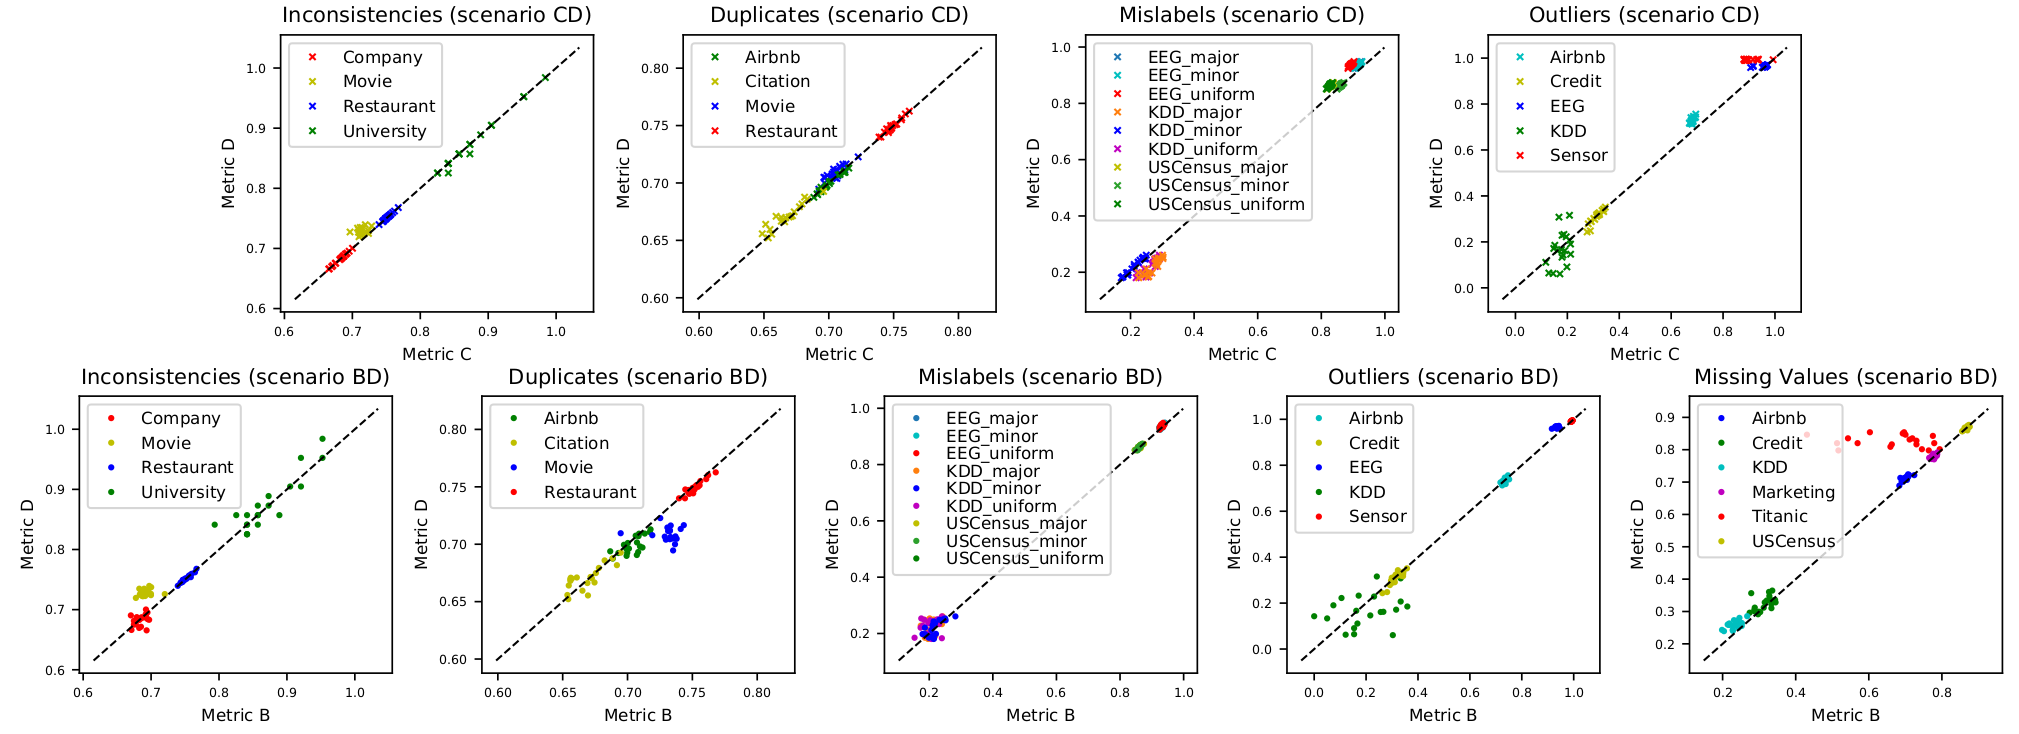
\includegraphics[angle=-90,scale=.3]{Test_Accuracy_Scores_in_Scenarios_BD_and_CD_of_20_Splits_for_Five_Error_Types}
	\caption{Test Accuracy Scores in Scenarios BD and CD of 20 Splits for Five Error Types}
	\label{fig:Test_Accuracy_Scores_in_Scenarios_BD_and_CD_of_20_Splits_for_Five_Error_Types}
\end{figure}

\begin{landscape}
\begin{table}[ht]
	\centering
	\caption{Benchmark Results(Organized by Query)}
	\label{tab:benchmark-results}
	\renewcommand{\arraystretch}{2}	
	\def\arraystretch{1.7}
	\resizebox{\textwidth}{!}{%
	\begin{tabular}{|l|lllll|} 
		
		\hline
		\centering
		\multirow{2}{*}{Q1}                      
		
		& 
		\begin{tabular}{llll}
		 	\multicolumn{4}{l}{Q1(E=Inconsistencies)} \\ \hline
		 	\multicolumn{1}{|l|}{R} & \multicolumn{1}{l|}{P} & \multicolumn{1}{l|}{S} & \multicolumn{1}{l|}{N} \\ \hline
		 	\multicolumn{1}{|l|}{R1} & \multicolumn{1}{l|}{14.29\% (8)} & \multicolumn{1}{l|}{85.71\% (48)} & \multicolumn{1}{l|}{0\%(0)} \\ \hline
		 	\multicolumn{1}{|l|}{R2} & \multicolumn{1}{l|}{5.0\% (2)} & \multicolumn{1}{l|}{75.0\% (6)} & \multicolumn{1}{l|}{0\%(0)} \\ \hline
		 	\multicolumn{1}{|l|}{R3} & \multicolumn{1}{l|}{37.5\% (3)} & \multicolumn{1}{l|}{62.5\% (5)} & \multicolumn{1}{l|}{0\%(0)} \\ \hline
		 \end{tabular}						  								 							  
		& 										  	
		\begin{tabular}{llll}
			\multicolumn{4}{l}{Q1(E=Duplicates)} \\ \hline
			\multicolumn{1}{|l|}{R} & \multicolumn{1}{l|}{P} & \multicolumn{1}{l|}{S} & \multicolumn{1}{l|}{N} \\ \hline
			\multicolumn{1}{|l|}{R1} & \multicolumn{1}{l|}{17.86\% (10)} & \multicolumn{1}{l|}{71.43\% (40)} & \multicolumn{1}{l|}{10.71\% (6)} \\ \hline
			\multicolumn{1}{|l|}{R2} & \multicolumn{1}{l|}{12.5\% (1)} & \multicolumn{1}{l|}{62.5\% (5)} & \multicolumn{1}{l|}{25.0\% (2)} \\ \hline
			\multicolumn{1}{|l|}{R3} & \multicolumn{1}{l|}{25.0\% (2)} & \multicolumn{1}{l|}{50.0\% (4)} & \multicolumn{1}{l|}{25.0\% (2)} \\ \hline
		\end{tabular}											   								  	 
		& 
		\begin{tabular}{llll}
			\multicolumn{4}{l}{Q1(E=Mislabels)} \\ \hline
			\multicolumn{1}{|l|}{R} & \multicolumn{1}{l|}{P} & \multicolumn{1}{l|}{S} & \multicolumn{1}{l|}{N} \\ \hline
			\multicolumn{1}{|l|}{R1} & \multicolumn{1}{l|}{59.52\% (75)} & \multicolumn{1}{l|}{26.19\% (33)} & \multicolumn{1}{l|}{14.29\% (18)} \\ \hline
			\multicolumn{1}{|l|}{R2} & \multicolumn{1}{l|}{61.11\% (11)} & \multicolumn{1}{l|}{27.78\% (5)} & \multicolumn{1}{l|}{11.11\% (2)} \\ \hline
			\multicolumn{1}{|l|}{R3} & \multicolumn{1}{l|}{61.11\% (11)} & \multicolumn{1}{l|}{27.78\% (5)} & \multicolumn{1}{l|}{11.11\% (2)} \\ \hline
		\end{tabular}
		&
		\begin{tabular}{llll}
			\multicolumn{4}{l}{Q1(E=Outliers)} \\ \hline
			\multicolumn{1}{|l|}{R} & \multicolumn{1}{l|}{P} & \multicolumn{1}{l|}{S} & \multicolumn{1}{l|}{N} \\ \hline
			\multicolumn{1}{|l|}{R1} & \multicolumn{1}{l|}{31.55\% (265)} & \multicolumn{1}{l|}{57.02\% (479)} & \multicolumn{1}{l|}{11.43\% (96)} \\ \hline
			\multicolumn{1}{|l|}{R2} & \multicolumn{1}{l|}{33.33\% (40)} & \multicolumn{1}{l|}{60\% (72)} & \multicolumn{1}{l|}{6.67\% (8)} \\ \hline
			\multicolumn{1}{|l|}{R3} & \multicolumn{1}{l|}{30\% (3)} & \multicolumn{1}{l|}{70\% (7)} & \multicolumn{1}{l|}{0\% (0)} \\ \hline
		\end{tabular}
		&
		\begin{tabular}{llll}
			\multicolumn{4}{l}{Q1(E=Missing Values)} \\ \hline
			\multicolumn{1}{|l|}{R} & \multicolumn{1}{l|}{P} & \multicolumn{1}{l|}{S} & \multicolumn{1}{l|}{N} \\ \hline
			\multicolumn{1}{|l|}{R1} & \multicolumn{1}{l|}{61.51\% (155)} & \multicolumn{1}{l|}{34.92\% (88)} & \multicolumn{1}{l|}{3.57\% (9)} \\ \hline
			\multicolumn{1}{|l|}{R2} & \multicolumn{1}{l|}{50.00\% (18)} & \multicolumn{1}{l|}{50.00\% (18)} & \multicolumn{1}{l|}{0.00\% (0)} \\ \hline
			\multicolumn{1}{|l|}{R3} & \multicolumn{1}{l|}{50.00\% (3)} & \multicolumn{1}{l|}{50.00\% (3)} & \multicolumn{1}{l|}{0.00\% (0)} \\ \hline
		\end{tabular}
		
		\\							                         
		& 
		& 
		& 
		&                      
		&
		
		\\ 
		
		\cline{1-1}
		\centering
		\multirow{2}{*}{Q2}
		&   
		\begin{tabular}{llll}
			\multicolumn{4}{l}{Q2(E=Inconsistencies)} \\ \hline
			\multicolumn{1}{|l|}{R} & \multicolumn{1}{l|}{Scenario} & \multicolumn{1}{l|}{P} & \multicolumn{1}{l|}{S} \\ \hline
			\multicolumn{1}{|c|}{\multirow{2}{*}{R1}} & \multicolumn{1}{l|}{BD} & \multicolumn{1}{l|}{7.14\% (2)} & \multicolumn{1}{l|}{92.86\% (26)} \\ \cline{2-4} 
			\multicolumn{1}{|c|}{} & \multicolumn{1}{l|}{CD} & \multicolumn{1}{l|}{21.43\% (6)} & \multicolumn{1}{l|}{78.57\% (22)} \\ \hline
			\multicolumn{1}{|l|}{\multirow{2}{*}{R2}} & \multicolumn{1}{l|}{BD} & \multicolumn{1}{l|}{25.0\% (1)} & \multicolumn{1}{l|}{75.0\% (3)} \\ \cline{2-4} 
			\multicolumn{1}{|l|}{} & \multicolumn{1}{l|}{CD} & \multicolumn{1}{l|}{25.0\% (1)} & \multicolumn{1}{l|}{75.0\% (3)} \\ \hline
			\multicolumn{1}{|l|}{\multirow{2}{*}{R3}} & \multicolumn{1}{l|}{BD} & \multicolumn{1}{l|}{25.0\% (1)} & \multicolumn{1}{l|}{75.0\% (3)} \\ \cline{2-4} 
			\multicolumn{1}{|l|}{} & \multicolumn{1}{l|}{CD} & \multicolumn{1}{l|}{50.0\% (2)} & \multicolumn{1}{l|}{50.0\% (2)} \\ \hline
		\end{tabular}
		&   
		\begin{tabular}{lllll}
			\multicolumn{5}{l}{Q2(E=Duplicates)} \\ \hline
			\multicolumn{1}{|l|}{R} & \multicolumn{1}{l|}{Scenario} & \multicolumn{1}{l|}{P} & \multicolumn{1}{l|}{S} & \multicolumn{1}{l|}{N} \\ \hline
			\multicolumn{1}{|c|}{\multirow{2}{*}{R1}} & \multicolumn{1}{l|}{BD} & \multicolumn{1}{l|}{10.71\% (3)} & \multicolumn{1}{l|}{75.0\% (21)} & \multicolumn{1}{l|}{14.29\% (4)} \\ \cline{2-5} 
			\multicolumn{1}{|c|}{} & \multicolumn{1}{l|}{CD} & \multicolumn{1}{l|}{25.0\% (7)} & \multicolumn{1}{l|}{67.86\% (19)} & \multicolumn{1}{l|}{7.14\% (2)} \\ \hline
			\multicolumn{1}{|l|}{\multirow{2}{*}{R2}} & \multicolumn{1}{l|}{BD} & \multicolumn{1}{l|}{0.0\% (0)} & \multicolumn{1}{l|}{50.0\% (2)} & \multicolumn{1}{l|}{50.0\% (2)} \\ \cline{2-5} 
			\multicolumn{1}{|l|}{} & \multicolumn{1}{l|}{CD} & \multicolumn{1}{l|}{25.0\% (1)} & \multicolumn{1}{l|}{75.0\% (3)} & \multicolumn{1}{l|}{0.0\% (0)} \\ \hline
			\multicolumn{1}{|l|}{\multirow{2}{*}{R3}} & \multicolumn{1}{l|}{BD} & \multicolumn{1}{l|}{0.0\% (0)} & \multicolumn{1}{l|}{50.0\% (2)} & \multicolumn{1}{l|}{50.0\% (2)} \\ \cline{2-5} 
			\multicolumn{1}{|l|}{} & \multicolumn{1}{l|}{CD} & \multicolumn{1}{l|}{50.0\% (2)} & \multicolumn{1}{l|}{50.0\% (2)} & \multicolumn{1}{l|}{0.0\% (0)} \\ \hline
		\end{tabular}
		& 
		\begin{tabular}{lllll}
			\multicolumn{5}{l}{Q2(E=Mislabels)} \\ \hline
			\multicolumn{1}{|l|}{R} & \multicolumn{1}{l|}{Scenario} & \multicolumn{1}{l|}{P} & \multicolumn{1}{l|}{S} & \multicolumn{1}{l|}{N} \\ \hline
			\multicolumn{1}{|c|}{\multirow{2}{*}{R1}} & \multicolumn{1}{l|}{BD} & \multicolumn{1}{l|}{50.79\% (32)} & \multicolumn{1}{l|}{49.21\% (31)} & \multicolumn{1}{l|}{0.0\% (0)} \\ \cline{2-5} 
			\multicolumn{1}{|c|}{} & \multicolumn{1}{l|}{CD} & \multicolumn{1}{l|}{68.25\% (43)} & \multicolumn{1}{l|}{3.17\% (2)} & \multicolumn{1}{l|}{28.57\% (18)} \\ \hline
			\multicolumn{1}{|l|}{\multirow{2}{*}{R2}} & \multicolumn{1}{l|}{BD} & \multicolumn{1}{l|}{44.44\% (4)} & \multicolumn{1}{l|}{55.56\% (5)} & \multicolumn{1}{l|}{0.0\% (0)} \\ \cline{2-5} 
			\multicolumn{1}{|l|}{} & \multicolumn{1}{l|}{CD} & \multicolumn{1}{l|}{77.78\% (7)} & \multicolumn{1}{l|}{0.0\% (0)} & \multicolumn{1}{l|}{22.22\% (2)} \\ \hline
			\multicolumn{1}{|l|}{\multirow{2}{*}{R3}} & \multicolumn{1}{l|}{BD} & \multicolumn{1}{l|}{44.44\% (4)} & \multicolumn{1}{l|}{55.56\% (5)} & \multicolumn{1}{l|}{0.0\% (0)} \\ \cline{2-5} 
			\multicolumn{1}{|l|}{} & \multicolumn{1}{l|}{CD} & \multicolumn{1}{l|}{77.78\% (7)} & \multicolumn{1}{l|}{0.0\% (0)} & \multicolumn{1}{l|}{22.22\% (2)} \\ \hline
		\end{tabular} 
		&
		\begin{tabular}{lllll}
			\multicolumn{5}{l}{Q2(E=Outliers)} \\ \hline
			\multicolumn{1}{|l|}{R} & \multicolumn{1}{l|}{Scenario} & \multicolumn{1}{l|}{P} & \multicolumn{1}{l|}{S} & \multicolumn{1}{l|}{N} \\ \hline
			\multicolumn{1}{|c|}{\multirow{2}{*}{R1}} & \multicolumn{1}{l|}{BD} & \multicolumn{1}{l|}{50.79\% (32)} & \multicolumn{1}{l|}{49.21\% (31)} & \multicolumn{1}{l|}{0.0\% (0)} \\ \cline{2-5} 
			\multicolumn{1}{|c|}{} & \multicolumn{1}{l|}{CD} & \multicolumn{1}{l|}{68.25\% (43)} & \multicolumn{1}{l|}{3.17\% (2)} & \multicolumn{1}{l|}{28.57\% (18)} \\ \hline
			\multicolumn{1}{|l|}{\multirow{2}{*}{R2}} & \multicolumn{1}{l|}{BD} & \multicolumn{1}{l|}{44.44\% (4)} & \multicolumn{1}{l|}{55.56\% (5)} & \multicolumn{1}{l|}{0.0\% (0)} \\ \cline{2-5} 
			\multicolumn{1}{|l|}{} & \multicolumn{1}{l|}{CD} & \multicolumn{1}{l|}{77.78\% (7)} & \multicolumn{1}{l|}{0.0\% (0)} & \multicolumn{1}{l|}{22.22\% (2)} \\ \hline
			\multicolumn{1}{|l|}{\multirow{2}{*}{R3}} & \multicolumn{1}{l|}{BD} & \multicolumn{1}{l|}{44.44\% (4)} & \multicolumn{1}{l|}{55.56\% (5)} & \multicolumn{1}{l|}{0.0\% (0)} \\ \cline{2-5} 
			\multicolumn{1}{|l|}{} & \multicolumn{1}{l|}{CD} & \multicolumn{1}{l|}{77.78\% (7)} & \multicolumn{1}{l|}{0.0\% (0)} & \multicolumn{1}{l|}{22.22\% (2)} \\ \hline
		\end{tabular}
		&

		\\
		&   
		&   
		&
		&                        
		&
		
		\\ 
		\cline{1-1}
		\multirow{2}{*}{Q3} 
		&   
		\begin{tabular}{clll}
			\multicolumn{4}{l}{Q3(E=Inconsistencies)} \\ \hline
			\multicolumn{1}{|l|}{R} & \multicolumn{1}{l|}{Model} & \multicolumn{1}{l|}{P} & \multicolumn{1}{l|}{S} \\ \hline
			\multicolumn{1}{|c|}{\multirow{7}{*}{R1}} & \multicolumn{1}{l|}{AdaBoost} & \multicolumn{1}{l|}{12.5\% (1)} & \multicolumn{1}{l|}{87.5\% (7)} \\ \cline{2-4} 
			\multicolumn{1}{|c|}{} & \multicolumn{1}{l|}{Decision Tree} & \multicolumn{1}{l|}{0.0\% (0)} & \multicolumn{1}{l|}{100.0\% (8)} \\ \cline{2-4} 
			\multicolumn{1}{|c|}{} & \multicolumn{1}{l|}{KNN} & \multicolumn{1}{l|}{25.0\% (2)} & \multicolumn{1}{l|}{75.0\% (6)} \\ \cline{2-4} 
			\multicolumn{1}{|c|}{} & \multicolumn{1}{l|}{Logistic Regression} & \multicolumn{1}{l|}{12.5\% (1)} & \multicolumn{1}{l|}{87.5\% (7)} \\ \cline{2-4} 
			\multicolumn{1}{|c|}{} & \multicolumn{1}{l|}{Naive Bayes} & \multicolumn{1}{l|}{12.5\% (1)} & \multicolumn{1}{l|}{87.5\% (7)} \\ \cline{2-4} 
			\multicolumn{1}{|c|}{} & \multicolumn{1}{l|}{Random Forest} & \multicolumn{1}{l|}{25.0\% (2)} & \multicolumn{1}{l|}{75.0\% (6)} \\ \cline{2-4} 
			\multicolumn{1}{|c|}{} & \multicolumn{1}{l|}{XGBoost} & \multicolumn{1}{l|}{12.5\% (1)} & \multicolumn{1}{l|}{87.5\% (7)} \\ \hline
		\end{tabular}
		&   
		\begin{tabular}{cllll}
			\multicolumn{5}{l}{Q3(E=Duplicates)} \\ \hline
			\multicolumn{1}{|l|}{R} & \multicolumn{1}{l|}{Model} & \multicolumn{1}{l|}{P} & \multicolumn{1}{l|}{S} & \multicolumn{1}{l|}{N} \\ \hline
			\multicolumn{1}{|c|}{\multirow{7}{*}{R1}} & \multicolumn{1}{l|}{AdaBoost} & \multicolumn{1}{l|}{25.0\% (2)} & \multicolumn{1}{l|}{75.0\% (6)} & \multicolumn{1}{l|}{0.0\% (0)} \\ \cline{2-5} 
			\multicolumn{1}{|c|}{} & \multicolumn{1}{l|}{Decision Tree} & \multicolumn{1}{l|}{0.0\% (0)} & \multicolumn{1}{l|}{100.0\% (8)} & \multicolumn{1}{l|}{0.0\% (0)} \\ \cline{2-5} 
			\multicolumn{1}{|c|}{} & \multicolumn{1}{l|}{KNN} & \multicolumn{1}{l|}{12.5\% (1)} & \multicolumn{1}{l|}{87.5\% (7)} & \multicolumn{1}{l|}{0.0\% (0)} \\ \cline{2-5} 
			\multicolumn{1}{|c|}{} & \multicolumn{1}{l|}{Logistic Regression} & \multicolumn{1}{l|}{25.0\% (2)} & \multicolumn{1}{l|}{62.5\% (5)} & \multicolumn{1}{l|}{12.5\% (1)} \\ \cline{2-5} 
			\multicolumn{1}{|c|}{} & \multicolumn{1}{l|}{Naive Bayes} & \multicolumn{1}{l|}{37.5\% (3)} & \multicolumn{1}{l|}{50.0\% (4)} & \multicolumn{1}{l|}{12.5\% (1)} \\ \cline{2-5} 
			\multicolumn{1}{|c|}{} & \multicolumn{1}{l|}{Random Forest} & \multicolumn{1}{l|}{12.5\% (1)} & \multicolumn{1}{l|}{62.5\% (5)} & \multicolumn{1}{l|}{25.0\% (2)} \\ \cline{2-5} 
			\multicolumn{1}{|c|}{} & \multicolumn{1}{l|}{XGBoost} & \multicolumn{1}{l|}{12.5\% (1)} & \multicolumn{1}{l|}{62.5\% (5)} & \multicolumn{1}{l|}{25.0\% (2)} \\ \hline
		\end{tabular}
		&               
		\begin{tabular}{cllll}
			\multicolumn{5}{l}{Q3(E=Mislabels)} \\ \hline
			\multicolumn{1}{|l|}{R} & \multicolumn{1}{l|}{Model} & \multicolumn{1}{l|}{P} & \multicolumn{1}{l|}{S} & \multicolumn{1}{l|}{N} \\ \hline
			\multicolumn{1}{|c|}{\multirow{7}{*}{R1}} & \multicolumn{1}{l|}{AdaBoost} & \multicolumn{1}{l|}{77.78\% (14)} & \multicolumn{1}{l|}{11.11\% (2)} & \multicolumn{1}{l|}{11.11\% (2)} \\ \cline{2-5} 
			\multicolumn{1}{|c|}{} & \multicolumn{1}{l|}{Decision Tree} & \multicolumn{1}{l|}{66.67\% (12)} & \multicolumn{1}{l|}{22.22\% (4)} & \multicolumn{1}{l|}{11.11\% (2)} \\ \cline{2-5} 
			\multicolumn{1}{|c|}{} & \multicolumn{1}{l|}{KNN} & \multicolumn{1}{l|}{50.0\% (9)} & \multicolumn{1}{l|}{38.89\% (7)} & \multicolumn{1}{l|}{11.11\% (2)} \\ \cline{2-5} 
			\multicolumn{1}{|c|}{} & \multicolumn{1}{l|}{Logistic Regression} & \multicolumn{1}{l|}{55.56\% (10)} & \multicolumn{1}{l|}{33.33\% (6)} & \multicolumn{1}{l|}{11.11\% (2)} \\ \cline{2-5} 
			\multicolumn{1}{|c|}{} & \multicolumn{1}{l|}{Naive Bayes} & \multicolumn{1}{l|}{27.78\% (5)} & \multicolumn{1}{l|}{38.89\% (7)} & \multicolumn{1}{l|}{33.33\% (6)} \\ \cline{2-5} 
			\multicolumn{1}{|c|}{} & \multicolumn{1}{l|}{Random Forest} & \multicolumn{1}{l|}{61.11\% (11)} & \multicolumn{1}{l|}{27.78\% (5)} & \multicolumn{1}{l|}{11.11\% (2)} \\ \cline{2-5} 
			\multicolumn{1}{|c|}{} & \multicolumn{1}{l|}{XGBoost} & \multicolumn{1}{l|}{77.78\% (14)} & \multicolumn{1}{l|}{11.11\% (2)} & \multicolumn{1}{l|}{11.11\% (2)} \\ \hline
		\end{tabular}         
		&
		\begin{tabular}{cllll}
			\multicolumn{5}{l}{Q3(E=Outliers)} \\ \hline
			\multicolumn{1}{|l|}{R} & \multicolumn{1}{l|}{Model} & \multicolumn{1}{l|}{P} & \multicolumn{1}{l|}{S} & \multicolumn{1}{l|}{N} \\ \hline
			\multicolumn{1}{|c|}{\multirow{7}{*}{R1}} & \multicolumn{1}{l|}{AdaBoost} & \multicolumn{1}{l|}{20\% (24)} & \multicolumn{1}{l|}{62.50\% (75)} & \multicolumn{1}{l|}{17.50\% (21)} \\ \cline{2-5} 
			\multicolumn{1}{|c|}{} & \multicolumn{1}{l|}{Decision Tree} & \multicolumn{1}{l|}{27.50\% (33)} & \multicolumn{1}{l|}{65.83\% (79)} & \multicolumn{1}{l|}{6.67\% (8)} \\ \cline{2-5} 
			\multicolumn{1}{|c|}{} & \multicolumn{1}{l|}{KNN} & \multicolumn{1}{l|}{50\% (60)} & \multicolumn{1}{l|}{44.17\% (53)} & \multicolumn{1}{l|}{5.83\% (7)} \\ \cline{2-5} 
			\multicolumn{1}{|c|}{} & \multicolumn{1}{l|}{Logistic Regression} & \multicolumn{1}{l|}{28.33\% (34)} & \multicolumn{1}{l|}{56.67\% (68)} & \multicolumn{1}{l|}{15\% (18)} \\ \cline{2-5} 
			\multicolumn{1}{|c|}{} & \multicolumn{1}{l|}{Naive Bayes} & \multicolumn{1}{l|}{34.17\% (41)} & \multicolumn{1}{l|}{58.33\% (70)} & \multicolumn{1}{l|}{7.5\% (9)} \\ \cline{2-5} 
			\multicolumn{1}{|c|}{} & \multicolumn{1}{l|}{Random Forest} & \multicolumn{1}{l|}{29.17\% (35)} & \multicolumn{1}{l|}{56.67\% (68)} & \multicolumn{1}{l|}{14.17\% (17)} \\ \cline{2-5} 
			\multicolumn{1}{|c|}{} & \multicolumn{1}{l|}{XGBoost} & \multicolumn{1}{l|}{31.67\% (38)} & \multicolumn{1}{l|}{55\% (66)} & \multicolumn{1}{l|}{13.33\% (16)} \\ \hline
		\end{tabular}
		&
		\begin{tabular}{cllll}
			\multicolumn{5}{l}{Q3(E=Missing Values)} \\ \hline
			\multicolumn{1}{|l|}{R} & \multicolumn{1}{l|}{Model} & \multicolumn{1}{l|}{P} & \multicolumn{1}{l|}{S} & \multicolumn{1}{l|}{N} \\ \hline
			\multicolumn{1}{|c|}{\multirow{7}{*}{R1}} & \multicolumn{1}{l|}{AdaBoost} & \multicolumn{1}{l|}{20\% (24)} & \multicolumn{1}{l|}{62.50\% (75)} & \multicolumn{1}{l|}{17.50\% (21)} \\ \cline{2-5} 
			\multicolumn{1}{|c|}{} & \multicolumn{1}{l|}{Decision Tree} & \multicolumn{1}{l|}{27.50\% (33)} & \multicolumn{1}{l|}{65.83\% (79)} & \multicolumn{1}{l|}{6.67\% (8)} \\ \cline{2-5} 
			\multicolumn{1}{|c|}{} & \multicolumn{1}{l|}{KNN} & \multicolumn{1}{l|}{50\% (60)} & \multicolumn{1}{l|}{44.17\% (53)} & \multicolumn{1}{l|}{5.83\% (7)} \\ \cline{2-5} 
			\multicolumn{1}{|c|}{} & \multicolumn{1}{l|}{Logistic Regression} & \multicolumn{1}{l|}{28.33\% (34)} & \multicolumn{1}{l|}{56.67\% (68)} & \multicolumn{1}{l|}{15\% (18)} \\ \cline{2-5} 
			\multicolumn{1}{|c|}{} & \multicolumn{1}{l|}{Naive Bayes} & \multicolumn{1}{l|}{34.17\% (41)} & \multicolumn{1}{l|}{58.33\% (70)} & \multicolumn{1}{l|}{7.5\% (9)} \\ \cline{2-5} 
			\multicolumn{1}{|c|}{} & \multicolumn{1}{l|}{Random Forest} & \multicolumn{1}{l|}{29.17\% (35)} & \multicolumn{1}{l|}{56.67\% (68)} & \multicolumn{1}{l|}{14.17\% (17)} \\ \cline{2-5} 
			\multicolumn{1}{|c|}{} & \multicolumn{1}{l|}{XGBoost} & \multicolumn{1}{l|}{31.67\% (38)} & \multicolumn{1}{l|}{55\% (66)} & \multicolumn{1}{l|}{13.33\% (16)} \\ \hline
		\end{tabular}
		\\            
		
		&   
		&   
		&
		&                       
		&
		
		\\ 
		\cline{1-1}
		\multirow{2}{*}{Q4}                       
		
		&   
		\begin{tabular}{lllll}
			\multicolumn{5}{l}{Q4.1(E=Outliers)} \\ \hline
			\multicolumn{1}{|l|}{R} & \multicolumn{1}{l|}{Detect Method} & \multicolumn{1}{l|}{P} & \multicolumn{1}{l|}{S} & \multicolumn{1}{l|}{N} \\ \hline
			\multicolumn{1}{|c|}{\multirow{3}{*}{R1}} & \multicolumn{1}{l|}{IF} & \multicolumn{1}{l|}{32.14\% (90)} & \multicolumn{1}{l|}{47.14\% (132)} & \multicolumn{1}{l|}{20.71\% (58)} \\ \cline{2-5} 
			\multicolumn{1}{|c|}{} & \multicolumn{1}{l|}{IQR} & \multicolumn{1}{l|}{50.71\% (142)} & \multicolumn{1}{l|}{38.21\% (107)} & \multicolumn{1}{l|}{11.07\% (31)} \\ \cline{2-5} 
			\multicolumn{1}{|c|}{} & \multicolumn{1}{l|}{SD} & \multicolumn{1}{l|}{11.79\% (33)} & \multicolumn{1}{l|}{85.71\% (240)} & \multicolumn{1}{l|}{2.50\% (7)} \\ \hline
			\multicolumn{1}{|l|}{\multirow{3}{*}{R2}} & \multicolumn{1}{l|}{IF} & \multicolumn{1}{l|}{32.50\% (13)} & \multicolumn{1}{l|}{60\% (24)} & \multicolumn{1}{l|}{7.50\% (3)} \\ \cline{2-5} 
			\multicolumn{1}{|l|}{} & \multicolumn{1}{l|}{IQR} & \multicolumn{1}{l|}{52.50\% (21)} & \multicolumn{1}{l|}{35\% (14)} & \multicolumn{1}{l|}{12.50\% (5)} \\ \cline{2-5} 
			\multicolumn{1}{|l|}{} & \multicolumn{1}{l|}{SD} & \multicolumn{1}{l|}{15\% (6)} & \multicolumn{1}{l|}{85\% (34)} & \multicolumn{1}{l|}{0\% (0)} \\ \hline
		\end{tabular}
		&   
		\begin{tabular}{lllll}
			\multicolumn{5}{l}{Q4.2(E=Outliers)} \\ \hline
			\multicolumn{1}{|l|}{R} & \multicolumn{1}{l|}{Repair Method} & \multicolumn{1}{l|}{P} & \multicolumn{1}{l|}{S} & \multicolumn{1}{l|}{N} \\ \hline
			\multicolumn{1}{|c|}{\multirow{4}{*}{R1}} & \multicolumn{1}{l|}{Delete} & \multicolumn{1}{l|}{32.86\% (69)} & \multicolumn{1}{l|}{50.48\% (106)} & \multicolumn{1}{l|}{16.67\% (35)} \\ \cline{2-5} 
			\multicolumn{1}{|c|}{} & \multicolumn{1}{l|}{Mean Imputation} & \multicolumn{1}{l|}{31.90\% (67)} & \multicolumn{1}{l|}{60.95\% (128)} & \multicolumn{1}{l|}{7.14\% (15)} \\ \cline{2-5} 
			\multicolumn{1}{|c|}{} & \multicolumn{1}{l|}{Mode Imputation} & \multicolumn{1}{l|}{30.95\% (65)} & \multicolumn{1}{l|}{57.14\% (120)} & \multicolumn{1}{l|}{11.90\% (25)} \\ \cline{2-5} 
			\multicolumn{1}{|c|}{} & \multicolumn{1}{l|}{Median Imputation} & \multicolumn{1}{l|}{30.48\% (64)} & \multicolumn{1}{l|}{59.52\% (125)} & \multicolumn{1}{l|}{10.00\% (21)} \\ \hline
			\multicolumn{1}{|l|}{\multirow{4}{*}{R2}} & \multicolumn{1}{l|}{Delete} & \multicolumn{1}{l|}{33.33\% (10)} & \multicolumn{1}{l|}{53.33\% (16)} & \multicolumn{1}{l|}{13.33\% (4)} \\ \cline{2-5} 
			\multicolumn{1}{|l|}{} & \multicolumn{1}{l|}{Mean Imputation} & \multicolumn{1}{l|}{33.33\% (10)} & \multicolumn{1}{l|}{63.33\% (19)} & \multicolumn{1}{l|}{3.33\% (1)} \\ \cline{2-5} 
			\multicolumn{1}{|l|}{} & \multicolumn{1}{l|}{Mode Imputation} & \multicolumn{1}{l|}{30.00\% (9)} & \multicolumn{1}{l|}{63.33\% (19)} & \multicolumn{1}{l|}{6.67\% (2)} \\ \cline{2-5} 
			\multicolumn{1}{|l|}{} & \multicolumn{1}{l|}{Median Imputation} & \multicolumn{1}{l|}{36.67\% (11)} & \multicolumn{1}{l|}{60.00\% (18)} & \multicolumn{1}{l|}{3.33\% (1)} \\ \hline
		\end{tabular}
		&
		\begin{tabular}{lllll}
			\multicolumn{5}{l}{Q4.2(E=Missing Values)} \\ \hline
			\multicolumn{1}{|l|}{R} & \multicolumn{1}{l|}{Imputation Method} & \multicolumn{1}{l|}{P} & \multicolumn{1}{l|}{S} & \multicolumn{1}{l|}{N} \\ \hline
			\multicolumn{1}{|c|}{\multirow{6}{*}{R1}} & \multicolumn{1}{l|}{Mean Dummy} & \multicolumn{1}{l|}{54.76\% (23)} & \multicolumn{1}{l|}{40.48\% (17)} & \multicolumn{1}{l|}{4.76\% (2)} \\ \cline{2-5} 
			\multicolumn{1}{|c|}{} & \multicolumn{1}{l|}{Median Dummy} & \multicolumn{1}{l|}{59.52\% (25)} & \multicolumn{1}{l|}{35.71\% (15)} & \multicolumn{1}{l|}{4.76\% (2)} \\ \cline{2-5} 
			\multicolumn{1}{|c|}{} & \multicolumn{1}{l|}{Mode Dummy} & \multicolumn{1}{l|}{64.29\% (27)} & \multicolumn{1}{l|}{30.95\% (13)} & \multicolumn{1}{l|}{4.76\% (2)} \\ \cline{2-5} 
			\multicolumn{1}{|c|}{} & \multicolumn{1}{l|}{Mean Mode} & \multicolumn{1}{l|}{64.29\% (27)} & \multicolumn{1}{l|}{33.33\% (14)} & \multicolumn{1}{l|}{2.38\% (1)} \\ \cline{2-5} 
			\multicolumn{1}{|c|}{} & \multicolumn{1}{l|}{Median Mode} & \multicolumn{1}{l|}{61.90\% (26)} & \multicolumn{1}{l|}{35.71\% (15)} & \multicolumn{1}{l|}{2.38\% (1)} \\ \cline{2-5} 
			\multicolumn{1}{|c|}{} & \multicolumn{1}{l|}{Mode Mode} & \multicolumn{1}{l|}{64.29\% (27)} & \multicolumn{1}{l|}{33.33\% (14)} & \multicolumn{1}{l|}{2.38\% (1)} \\ \hline
			\multicolumn{1}{|l|}{\multirow{6}{*}{R2}} & \multicolumn{1}{l|}{Mean Dummy} & \multicolumn{1}{l|}{50.00\% (3)} & \multicolumn{1}{l|}{50.00\% (3)} & \multicolumn{1}{l|}{0.00\% (0)} \\ \cline{2-5} 
			\multicolumn{1}{|l|}{} & \multicolumn{1}{l|}{Median Dummy} & \multicolumn{1}{l|}{50.00\% (3)} & \multicolumn{1}{l|}{50.00\% (3)} & \multicolumn{1}{l|}{0.00\% (0)} \\ \cline{2-5} 
			\multicolumn{1}{|l|}{} & \multicolumn{1}{l|}{Mode Dummy} & \multicolumn{1}{l|}{50.00\% (3)} & \multicolumn{1}{l|}{50.00\% (3)} & \multicolumn{1}{l|}{0.00\% (0)} \\ \cline{2-5} 
			\multicolumn{1}{|l|}{} & \multicolumn{1}{l|}{Mean Mode} & \multicolumn{1}{l|}{50.00\% (3)} & \multicolumn{1}{l|}{50.00\% (3)} & \multicolumn{1}{l|}{0.00\% (0)} \\ \cline{2-5} 
			\multicolumn{1}{|l|}{} & \multicolumn{1}{l|}{Median Mode} & \multicolumn{1}{l|}{50.00\% (3)} & \multicolumn{1}{l|}{50.00\% (3)} & \multicolumn{1}{l|}{0.00\% (0)} \\ \cline{2-5} 
			\multicolumn{1}{|l|}{} & \multicolumn{1}{l|}{Mode Mode} & \multicolumn{1}{l|}{50.00\% (3)} & \multicolumn{1}{l|}{50.00\% (3)} & \multicolumn{1}{l|}{0.00\% (0)} \\ \hline
		\end{tabular}
		&                        
		&
		
		\\
		
		&   
		&   
		&
		&                        
		&
		
		\\ 
		\cline{1-1}
		\multirow{2}{*}{Q5}                       
		
		&   
		\begin{tabular}{llll}
			\multicolumn{4}{l}{Q5(E=Inconsistencies)} \\ \hline
			\multicolumn{1}{|l|}{R} & \multicolumn{1}{l|}{Dataset} & \multicolumn{1}{l|}{P} & \multicolumn{1}{l|}{S} \\ \hline
			\multicolumn{1}{|c|}{\multirow{4}{*}{R1}} & \multicolumn{1}{l|}{Company} & \multicolumn{1}{l|}{28.57\% (4)} & \multicolumn{1}{l|}{71.43\% (10)} \\ \cline{2-4} 
			\multicolumn{1}{|c|}{} & \multicolumn{1}{l|}{Movie} & \multicolumn{1}{l|}{21.43\% (3)} & \multicolumn{1}{l|}{78.57\% (11)} \\ \cline{2-4} 
			\multicolumn{1}{|c|}{} & \multicolumn{1}{l|}{Restaurant} & \multicolumn{1}{l|}{0.0\% (0)} & \multicolumn{1}{l|}{100.0\% (14)} \\ \cline{2-4} 
			\multicolumn{1}{|c|}{} & \multicolumn{1}{l|}{University} & \multicolumn{1}{l|}{7.14\% (1)} & \multicolumn{1}{l|}{92.86\% (13)} \\ \hline
			\multicolumn{1}{|l|}{\multirow{4}{*}{R2}} & \multicolumn{1}{l|}{Company} & \multicolumn{1}{l|}{0.0\% (0)} & \multicolumn{1}{l|}{100.0\% (2)} \\ \cline{2-4} 
			\multicolumn{1}{|l|}{} & \multicolumn{1}{l|}{Movie} & \multicolumn{1}{l|}{100.0\% (2)} & \multicolumn{1}{l|}{0.0\% (0)} \\ \cline{2-4} 
			\multicolumn{1}{|l|}{} & \multicolumn{1}{l|}{Restaurant} & \multicolumn{1}{l|}{0.0\% (0)} & \multicolumn{1}{l|}{100.0\% (2)} \\ \cline{2-4} 
			\multicolumn{1}{|l|}{} & \multicolumn{1}{l|}{University} & \multicolumn{1}{l|}{0.0\% (0)} & \multicolumn{1}{l|}{100.0\% (2)} \\ \hline
			\multicolumn{1}{|l|}{\multirow{4}{*}{R3}} & \multicolumn{1}{l|}{Company} & \multicolumn{1}{l|}{0.0\% (0)} & \multicolumn{1}{l|}{100.0\% (2)} \\ \cline{2-4} 
			\multicolumn{1}{|l|}{} & \multicolumn{1}{l|}{Movie} & \multicolumn{1}{l|}{100.0\% (2)} & \multicolumn{1}{l|}{0.0\% (0)} \\ \cline{2-4} 
			\multicolumn{1}{|l|}{} & \multicolumn{1}{l|}{Restaurant} & \multicolumn{1}{l|}{50.0\% (1)} & \multicolumn{1}{l|}{50.0\% (1)} \\ \cline{2-4} 
			\multicolumn{1}{|l|}{} & \multicolumn{1}{l|}{University} & \multicolumn{1}{l|}{0.0\% (0)} & \multicolumn{1}{l|}{100.0\% (2)} \\ \hline
		\end{tabular}
		&   
		\begin{tabular}{lllll}
			\multicolumn{5}{l}{Q5(E=Duplicates)} \\ \hline
			\multicolumn{1}{|l|}{R} & \multicolumn{1}{l|}{Dataset} & \multicolumn{1}{l|}{P} & \multicolumn{1}{l|}{S} & \multicolumn{1}{l|}{N} \\ \hline
			\multicolumn{1}{|c|}{\multirow{4}{*}{R1}} & \multicolumn{1}{l|}{Airbnb} & \multicolumn{1}{l|}{0.0\% (0)} & \multicolumn{1}{l|}{85.71\% (12)} & \multicolumn{1}{l|}{14.29\% (2)} \\ \cline{2-5} 
			\multicolumn{1}{|c|}{} & \multicolumn{1}{l|}{Citation} & \multicolumn{1}{l|}{7.14\% (1)} & \multicolumn{1}{l|}{85.71\% (12)} & \multicolumn{1}{l|}{7.14\% (1)} \\ \cline{2-5} 
			\multicolumn{1}{|c|}{} & \multicolumn{1}{l|}{Movie} & \multicolumn{1}{l|}{64.29\% (9)} & \multicolumn{1}{l|}{28.57\% (4)} & \multicolumn{1}{l|}{7.14\% (1)} \\ \cline{2-5} 
			\multicolumn{1}{|c|}{} & \multicolumn{1}{l|}{Restaurant} & \multicolumn{1}{l|}{0.0\% (0)} & \multicolumn{1}{l|}{85.71\% (12)} & \multicolumn{1}{l|}{14.29\% (2)} \\ \hline
			\multicolumn{1}{|l|}{\multirow{4}{*}{R2}} & \multicolumn{1}{l|}{Airbnb} & \multicolumn{1}{l|}{0.0\% (0)} & \multicolumn{1}{l|}{100.0\% (2)} & \multicolumn{1}{l|}{0.0\% (0)} \\ \cline{2-5} 
			\multicolumn{1}{|l|}{} & \multicolumn{1}{l|}{Citation} & \multicolumn{1}{l|}{0.0\% (0)} & \multicolumn{1}{l|}{100.0\% (2)} & \multicolumn{1}{l|}{0.0\% (0)} \\ \cline{2-5} 
			\multicolumn{1}{|l|}{} & \multicolumn{1}{l|}{Movie} & \multicolumn{1}{l|}{50.0\% (1)} & \multicolumn{1}{l|}{0.0\% (0)} & \multicolumn{1}{l|}{50.0\% (1)} \\ \cline{2-5} 
			\multicolumn{1}{|l|}{} & \multicolumn{1}{l|}{Restaurant} & \multicolumn{1}{l|}{0.0\% (0)} & \multicolumn{1}{l|}{50.0\% (1)} & \multicolumn{1}{l|}{50.0\% (1)} \\ \hline
			\multicolumn{1}{|l|}{\multirow{4}{*}{R3}} & \multicolumn{1}{l|}{Airbnb} & \multicolumn{1}{l|}{0.0\% (0)} & \multicolumn{1}{l|}{100.0\% (2)} & \multicolumn{1}{l|}{0.0\% (0)} \\ \cline{2-5} 
			\multicolumn{1}{|l|}{} & \multicolumn{1}{l|}{Citation} & \multicolumn{1}{l|}{50.0\% (1)} & \multicolumn{1}{l|}{50.0\% (1)} & \multicolumn{1}{l|}{0.0\% (0)} \\ \cline{2-5} 
			\multicolumn{1}{|l|}{} & \multicolumn{1}{l|}{Movie} & \multicolumn{1}{l|}{50.0\% (1)} & \multicolumn{1}{l|}{0.0\% (0)} & \multicolumn{1}{l|}{50.0\% (1)} \\ \cline{2-5} 
			\multicolumn{1}{|l|}{} & \multicolumn{1}{l|}{Restaurant} & \multicolumn{1}{l|}{0.0\% (0)} & \multicolumn{1}{l|}{50.0\% (1)} & \multicolumn{1}{l|}{50.0\% (1)} \\ \hline
		\end{tabular}
		& 
		\begin{tabular}{lllll}
			\multicolumn{5}{l}{Q5(E=Outliers)} \\ \hline
			\multicolumn{1}{|l|}{R} & \multicolumn{1}{l|}{Dataset} & \multicolumn{1}{l|}{P} & \multicolumn{1}{l|}{S} & \multicolumn{1}{l|}{N} \\ \hline
			\multicolumn{1}{|c|}{\multirow{4}{*}{R1}} & \multicolumn{1}{l|}{Airbnb} & \multicolumn{1}{l|}{0.0\% (0)} & \multicolumn{1}{l|}{85.71\% (12)} & \multicolumn{1}{l|}{14.29\% (2)} \\ \cline{2-5} 
			\multicolumn{1}{|c|}{} & \multicolumn{1}{l|}{Citation} & \multicolumn{1}{l|}{7.14\% (1)} & \multicolumn{1}{l|}{85.71\% (12)} & \multicolumn{1}{l|}{7.14\% (1)} \\ \cline{2-5} 
			\multicolumn{1}{|c|}{} & \multicolumn{1}{l|}{Movie} & \multicolumn{1}{l|}{64.29\% (9)} & \multicolumn{1}{l|}{28.57\% (4)} & \multicolumn{1}{l|}{7.14\% (1)} \\ \cline{2-5} 
			\multicolumn{1}{|c|}{} & \multicolumn{1}{l|}{Restaurant} & \multicolumn{1}{l|}{0.0\% (0)} & \multicolumn{1}{l|}{85.71\% (12)} & \multicolumn{1}{l|}{14.29\% (2)} \\ \hline
			\multicolumn{1}{|l|}{\multirow{4}{*}{R2}} & \multicolumn{1}{l|}{Airbnb} & \multicolumn{1}{l|}{0.0\% (0)} & \multicolumn{1}{l|}{100.0\% (2)} & \multicolumn{1}{l|}{0.0\% (0)} \\ \cline{2-5} 
			\multicolumn{1}{|l|}{} & \multicolumn{1}{l|}{Citation} & \multicolumn{1}{l|}{0.0\% (0)} & \multicolumn{1}{l|}{100.0\% (2)} & \multicolumn{1}{l|}{0.0\% (0)} \\ \cline{2-5} 
			\multicolumn{1}{|l|}{} & \multicolumn{1}{l|}{Movie} & \multicolumn{1}{l|}{50.0\% (1)} & \multicolumn{1}{l|}{0.0\% (0)} & \multicolumn{1}{l|}{50.0\% (1)} \\ \cline{2-5} 
			\multicolumn{1}{|l|}{} & \multicolumn{1}{l|}{Restaurant} & \multicolumn{1}{l|}{0.0\% (0)} & \multicolumn{1}{l|}{50.0\% (1)} & \multicolumn{1}{l|}{50.0\% (1)} \\ \hline
			\multicolumn{1}{|l|}{\multirow{4}{*}{R3}} & \multicolumn{1}{l|}{Airbnb} & \multicolumn{1}{l|}{0.0\% (0)} & \multicolumn{1}{l|}{100.0\% (2)} & \multicolumn{1}{l|}{0.0\% (0)} \\ \cline{2-5} 
			\multicolumn{1}{|l|}{} & \multicolumn{1}{l|}{Citation} & \multicolumn{1}{l|}{50.0\% (1)} & \multicolumn{1}{l|}{50.0\% (1)} & \multicolumn{1}{l|}{0.0\% (0)} \\ \cline{2-5} 
			\multicolumn{1}{|l|}{} & \multicolumn{1}{l|}{Movie} & \multicolumn{1}{l|}{50.0\% (1)} & \multicolumn{1}{l|}{0.0\% (0)} & \multicolumn{1}{l|}{50.0\% (1)} \\ \cline{2-5} 
			\multicolumn{1}{|l|}{} & \multicolumn{1}{l|}{Restaurant} & \multicolumn{1}{l|}{0.0\% (0)} & \multicolumn{1}{l|}{50.0\% (1)} & \multicolumn{1}{l|}{50.0\% (1)} \\ \hline
		\end{tabular}
		&   
		\begin{tabular}{lllll}
			\multicolumn{5}{l}{Q5(E=Missing Values)} \\ \hline
			\multicolumn{1}{|l|}{R} & \multicolumn{1}{l|}{Dataset} & \multicolumn{1}{l|}{P} & \multicolumn{1}{l|}{S} & \multicolumn{1}{l|}{N} \\ \hline
			\multicolumn{1}{|c|}{\multirow{5}{*}{R1}} & \multicolumn{1}{l|}{Airbnb} & \multicolumn{1}{l|}{23.21\% (39)} & \multicolumn{1}{l|}{70.83\% (119)} & \multicolumn{1}{l|}{5.95\% (10)} \\ \cline{2-5} 
			\multicolumn{1}{|c|}{} & \multicolumn{1}{l|}{Credit} & \multicolumn{1}{l|}{22.62\% (38)} & \multicolumn{1}{l|}{43.35\% (73)} & \multicolumn{1}{l|}{33.93\% (57)} \\ \cline{2-5} 
			\multicolumn{1}{|c|}{} & \multicolumn{1}{l|}{EEG} & \multicolumn{1}{l|}{60.12\% (101)} & \multicolumn{1}{l|}{33.93\% (57)} & \multicolumn{1}{l|}{5.95\% (10)} \\ \cline{2-5} 
			\multicolumn{1}{|c|}{} & \multicolumn{1}{l|}{KDD} & \multicolumn{1}{l|}{3.57\% (6)} & \multicolumn{1}{l|}{93.45\% (157)} & \multicolumn{1}{l|}{2.98\% (5)} \\ \cline{2-5} 
			\multicolumn{1}{|c|}{} & \multicolumn{1}{l|}{Sensor} & \multicolumn{1}{l|}{48.21\% (81)} & \multicolumn{1}{l|}{43.45\% (73)} & \multicolumn{1}{l|}{8.33\% (14)} \\ \hline
			\multicolumn{1}{|l|}{\multirow{5}{*}{R2}} & \multicolumn{1}{l|}{Airbnb} & \multicolumn{1}{l|}{37.50\% (9)} & \multicolumn{1}{l|}{62.50\%(15)} & \multicolumn{1}{l|}{0.0\% (0)} \\ \cline{2-5} 
			\multicolumn{1}{|l|}{} & \multicolumn{1}{l|}{Credit} & \multicolumn{1}{l|}{0.0\% (0)} & \multicolumn{1}{l|}{66.67\% (16)} & \multicolumn{1}{l|}{33.33\% (8)} \\ \cline{2-5} 
			\multicolumn{1}{|l|}{} & \multicolumn{1}{l|}{EEG} & \multicolumn{1}{l|}{79.17\% (19)} & \multicolumn{1}{l|}{20.83\% (5)} & \multicolumn{1}{l|}{0\% (0)} \\ \cline{2-5} 
			\multicolumn{1}{|l|}{} & \multicolumn{1}{l|}{KDD} & \multicolumn{1}{l|}{0.0\% (0)} & \multicolumn{1}{l|}{100\% (0)} & \multicolumn{1}{l|}{0\% (0)} \\ \cline{2-5} 
			\multicolumn{1}{|l|}{} & \multicolumn{1}{l|}{Sensor} & \multicolumn{1}{l|}{50\% (12)} & \multicolumn{1}{l|}{50\% (12)} & \multicolumn{1}{l|}{0\% (0)} \\ \hline
			\multicolumn{1}{|l|}{\multirow{5}{*}{R3}} & \multicolumn{1}{l|}{Airbnb} & \multicolumn{1}{l|}{50\% (1)} & \multicolumn{1}{l|}{50\% (1)} & \multicolumn{1}{l|}{0.0\% (0)} \\ \cline{2-5} 
			\multicolumn{1}{|l|}{} & \multicolumn{1}{l|}{Credit} & \multicolumn{1}{l|}{0\% (0)} & \multicolumn{1}{l|}{100\% (2)} & \multicolumn{1}{l|}{0.0\% (0)} \\ \cline{2-5} 
			\multicolumn{1}{|l|}{} & \multicolumn{1}{l|}{EEG} & \multicolumn{1}{l|}{50.0\% (1)} & \multicolumn{1}{l|}{50\% (1)} & \multicolumn{1}{l|}{0\% (0)} \\ \cline{2-5} 
			\multicolumn{1}{|l|}{} & \multicolumn{1}{l|}{KDD} & \multicolumn{1}{l|}{0.0\% (0)} & \multicolumn{1}{l|}{100\% (2)} & \multicolumn{1}{l|}{0\% (0)} \\ \cline{2-5} 
			\multicolumn{1}{|l|}{} & \multicolumn{1}{l|}{Sensor} & \multicolumn{1}{l|}{50\% (1)} & \multicolumn{1}{l|}{50\% (1)} & \multicolumn{1}{l|}{0\% (0)} \\ \hline
		\end{tabular}                    
	    &
	    \begin{tabular}{cllll}
	    	\multicolumn{5}{l}{Q5(E=Mislabels)} \\ \hline
	    	\multicolumn{1}{|l|}{R} & \multicolumn{1}{l|}{Dataset} & \multicolumn{1}{l|}{P} & \multicolumn{1}{l|}{S} & \multicolumn{1}{l|}{N} \\ \hline
	    	\multicolumn{1}{|c|}{\multirow{18}{*}{R1}} & \multicolumn{1}{l|}{EEG major} & \multicolumn{1}{l|}{78.57\% (11)} & \multicolumn{1}{l|}{14.29\% (2)} & \multicolumn{1}{l|}{7.14\% (1)} \\ \cline{2-5} 
	    	\multicolumn{1}{|c|}{} & \multicolumn{1}{l|}{EEG minor} & \multicolumn{1}{l|}{78.57\% (11)} & \multicolumn{1}{l|}{21.43\% (3)} & \multicolumn{1}{l|}{0.0\% (0)} \\ \cline{2-5} 
	    	\multicolumn{1}{|c|}{} & \multicolumn{1}{l|}{EEG uniform} & \multicolumn{1}{l|}{78.57\% (11)} & \multicolumn{1}{l|}{14.29\% (2)} & \multicolumn{1}{l|}{7.14\% (1)} \\ \cline{2-5} 
	    	\multicolumn{1}{|c|}{} & \multicolumn{1}{l|}{KDD major} & \multicolumn{1}{l|}{28.57\% (4)} & \multicolumn{1}{l|}{21.43\% (3)} & \multicolumn{1}{l|}{50.0\% (7)} \\ \cline{2-5} 
	    	\multicolumn{1}{|c|}{} & \multicolumn{1}{l|}{KDD minor} & \multicolumn{1}{l|}{50.0\% (7)} & \multicolumn{1}{l|}{50.0\% (7)} & \multicolumn{1}{l|}{0.0\% (0)} \\ \cline{2-5} 
	    	\multicolumn{1}{|c|}{} & \multicolumn{1}{l|}{KDD uniform} & \multicolumn{1}{l|}{35.71\% (5)} & \multicolumn{1}{l|}{14.29\% (2)} & \multicolumn{1}{l|}{50.0\% (7)} \\ \cline{2-5} 
	    	\multicolumn{1}{|c|}{} & \multicolumn{1}{l|}{USCensus major} & \multicolumn{1}{l|}{50.0\% (7)} & \multicolumn{1}{l|}{42.86\% (6)} & \multicolumn{1}{l|}{7.14\% (1)} \\ \cline{2-5} 
	    	\multicolumn{1}{|c|}{} & \multicolumn{1}{l|}{USCensus minor} & \multicolumn{1}{l|}{64.29\% (9)} & \multicolumn{1}{l|}{35.71\% (5)} & \multicolumn{1}{l|}{0.0\% (0)} \\ \cline{2-5} 
	    	\multicolumn{1}{|c|}{} & \multicolumn{1}{l|}{USCensus uniform} & \multicolumn{1}{l|}{71.43\% (10)} & \multicolumn{1}{l|}{21.43\% (3)} & \multicolumn{1}{l|}{7.14\% (1)} \\ \cline{2-5} 
	    	\multicolumn{1}{|c|}{} & \multicolumn{1}{l|}{EEG major} & \multicolumn{1}{l|}{100.0\% (2)} & \multicolumn{1}{l|}{0.0\% (0)} & \multicolumn{1}{l|}{0.0\% (0)} \\ \cline{2-5} 
	    	\multicolumn{1}{|c|}{} & \multicolumn{1}{l|}{EEG minor} & \multicolumn{1}{l|}{100.0\% (2)} & \multicolumn{1}{l|}{0.0\% (0)} & \multicolumn{1}{l|}{0.0\% (0)} \\ \cline{2-5} 
	    	\multicolumn{1}{|c|}{} & \multicolumn{1}{l|}{EEG uniform} & \multicolumn{1}{l|}{100.0\% (2)} & \multicolumn{1}{l|}{0.0\% (0)} & \multicolumn{1}{l|}{0.0\% (0)} \\ \cline{2-5} 
	    	\multicolumn{1}{|c|}{} & \multicolumn{1}{l|}{KDD major} & \multicolumn{1}{l|}{0.0\% (0)} & \multicolumn{1}{l|}{50.0\% (1)} & \multicolumn{1}{l|}{50.0\% (1)} \\ \cline{2-5} 
	    	\multicolumn{1}{|c|}{} & \multicolumn{1}{l|}{KDD minor} & \multicolumn{1}{l|}{50.0\% (1)} & \multicolumn{1}{l|}{50.0\% (1)} & \multicolumn{1}{l|}{0.0\% (0)} \\ \cline{2-5} 
	    	\multicolumn{1}{|c|}{} & \multicolumn{1}{l|}{KDD uniform} & \multicolumn{1}{l|}{0.0\% (0)} & \multicolumn{1}{l|}{50.0\% (1)} & \multicolumn{1}{l|}{50.0\% (1)} \\ \cline{2-5} 
	    	\multicolumn{1}{|c|}{} & \multicolumn{1}{l|}{USCensus major} & \multicolumn{1}{l|}{50.0\% (1)} & \multicolumn{1}{l|}{50.0\% (1)} & \multicolumn{1}{l|}{0.0\% (0)} \\ \cline{2-5} 
	    	\multicolumn{1}{|c|}{} & \multicolumn{1}{l|}{USCensus minor} & \multicolumn{1}{l|}{50.0\% (1)} & \multicolumn{1}{l|}{50.0\% (1)} & \multicolumn{1}{l|}{0.0\% (0)} \\ \cline{2-5} 
	    	\multicolumn{1}{|c|}{} & \multicolumn{1}{l|}{USCensus uniform} & \multicolumn{1}{l|}{100.0\% (2)} & \multicolumn{1}{l|}{0.0\% (0)} & \multicolumn{1}{l|}{0.0\% (0)} \\ \hline
	    	\multicolumn{1}{|l|}{\multirow{9}{*}{R2}} & \multicolumn{1}{l|}{EEG major} & \multicolumn{1}{l|}{100.0\% (2)} & \multicolumn{1}{l|}{0.0\% (0)} & \multicolumn{1}{l|}{0.0\% (0)} \\ \cline{2-5} 
	    	\multicolumn{1}{|l|}{} & \multicolumn{1}{l|}{EEG minor} & \multicolumn{1}{l|}{100.0\% (2)} & \multicolumn{1}{l|}{0.0\% (0)} & \multicolumn{1}{l|}{0.0\% (0)} \\ \cline{2-5} 
	    	\multicolumn{1}{|l|}{} & \multicolumn{1}{l|}{EEG uniform} & \multicolumn{1}{l|}{100.0\% (2)} & \multicolumn{1}{l|}{0.0\% (0)} & \multicolumn{1}{l|}{0.0\% (0)} \\ \cline{2-5} 
	    	\multicolumn{1}{|l|}{} & \multicolumn{1}{l|}{KDD major} & \multicolumn{1}{l|}{0.0\% (0)} & \multicolumn{1}{l|}{50.0\% (1)} & \multicolumn{1}{l|}{50.0\% (1)} \\ \cline{2-5} 
	    	\multicolumn{1}{|l|}{} & \multicolumn{1}{l|}{KDD minor} & \multicolumn{1}{l|}{50.0\% (1)} & \multicolumn{1}{l|}{50.0\% (1)} & \multicolumn{1}{l|}{0.0\% (0)} \\ \cline{2-5} 
	    	\multicolumn{1}{|l|}{} & \multicolumn{1}{l|}{KDD uniform} & \multicolumn{1}{l|}{0.0\% (0)} & \multicolumn{1}{l|}{50.0\% (1)} & \multicolumn{1}{l|}{50.0\% (1)} \\ \cline{2-5} 
	    	\multicolumn{1}{|l|}{} & \multicolumn{1}{l|}{USCensus major} & \multicolumn{1}{l|}{50.0\% (1)} & \multicolumn{1}{l|}{50.0\% (1)} & \multicolumn{1}{l|}{0.0\% (0)} \\ \cline{2-5} 
	    	\multicolumn{1}{|l|}{} & \multicolumn{1}{l|}{USCensus minor} & \multicolumn{1}{l|}{50.0\% (1)} & \multicolumn{1}{l|}{50.0\% (1)} & \multicolumn{1}{l|}{0.0\% (0)} \\ \cline{2-5} 
	    	\multicolumn{1}{|l|}{} & \multicolumn{1}{l|}{USCensus uniform} & \multicolumn{1}{l|}{100.0\% (2)} & \multicolumn{1}{l|}{0.0\% (0)} & \multicolumn{1}{l|}{0.0\% (0)} \\ \hline
	    \end{tabular}
	    \\
		&   
		&   
		& 
		&                        
		&
		
		\\
		\hline
	\end{tabular}
}
\end{table}
\end{landscape}

\begin{itemize}
	\item {
		\textbf{Q3:} Grouped by ML models, it is noticeable that all the ML models have demonstrated the same tendency in the impacts of data
		cleaning, as shown in Table \ref{tab:benchmark-results}: Q3(E=Inconsistencies). Again, there is no negative impact on ML performances that cleaning inconsistency can induce.
	}

	\item {
		\textbf{Q5:} At last, we group by datasets and provide a view on dataset
		choice and its influence on ML performance with data cleaning strategy incorporated. As shown in Table ~\ref{tab:benchmark-results}:(E=Inconsistencies),
		in general, the pattern holds that insignificant impact of cleaning inconsistency prevails; no negative impacts of cleaning inconsistency
		was found. It is probably due to the idiosyncrasy in the Movie
		dataset, which has 48\% of inconsistencies \footnote{We calculate the inconsistency of the datasets using the percentage of minority class. For instance, in the dataset Movie, we correct the values English and en under the variable “Language”. The value English takes 52\% in all the attribute values; the value en 48\%. We therefore replace en with English. This gives us an inconsistency rate of 48\%.} the improvement an auto ML/cleaning strategy tuner brings Hatton2019is 78.57\% in the direction of positive changes.
	}
\end{itemize}

\section{Duplicates} \label{sec:duplicates}

\begin{enumerate}
	\item {
		Cleaning duplicates is more likely to have insignificant
		impacts on ML and it is possible to produce negative impacts.
	}
	\item {
		With model selection, negative impacts caused by
		cleaning test set can be eliminated.
	}
\end{enumerate}

\begin{itemize}
	\item {
		\textbf{Q1:} From the query on flags shown in Table ~\ref{tab:benchmark-results}:Q1(E=Duplicates),
		it is unclear that if cleaning duplicates could bring either positive
		or negative impacts. In all the relations, the number of insignificant flags has the largest percentage compared with the positive
		and negative flags.
	}
	\item{
		\textbf{Q2:} Looking scenarios grouped by flags in Table ~\ref{tab:benchmark-results}: Q2 (E=Duplicates), using a clean test set with a clean training model (CD) is highly unlikely to result in negative changes of ML performance.
		Especially when we utilize an auto ML/data cleaning tuner, the negative impacts disappear. In the scenario BD, utilizing an ML/cleaning tuner does not decrease the chance of yielding negative impacts
		when we clean the duplicates. This observation is also made from
		the scatter plot on BD in Figure ~\ref{fig:Test_Accuracy_Scores_in_Scenarios_BD_and_CD_of_20_Splits_for_Five_Error_Types}, where there are more points with the “N” flag than the other two flags. The reason is due to the various duplication rates of features in the datasets, as we see when analyzing the results of Q5 below.
	}

	\item {
		\textbf{Q3}: We observe from Table ~\ref{tab:benchmark-results}:Q3(E=Duplicates) that for all the ML models, AdaBoost, KNN and Decision Tree tend to have no negative impact.
	}
	\item {
		\textbf{Q5}: The discrepancies of datasets affect the ML performances largely as we observe from Table ~\ref{tab:benchmark-results}:Q5(E=Duplicates). For the datasets “Airbnb” and “Citation”, the negative impacts could be
		dampened to zero if we add an auto ML/cleaning tuner. Yet for the datasets “Movie” and “Restaurant”, the negative impacts even increase after we use an auto ML/cleaning tuner. This might be due to the protocol of generating the duplicates, where we have combined the two sources of datasets and do not correlate the duplication rate
		with the class distribution. Finally, “Movie” has a duplication rate of 40\%, “Citation” 10\%, “Airbnb” 10\%, and “Restaurant” 10\%.
	}
\end{itemize}

\section{Mislabels} \label{sec:mislabels}

\begin{enumerate}
	\item {
		Cleaning mislabels are highly likely to have positive impacts on ML.
	}
	\item {
		Cleaning mislabels for models that have bad
		performances may produce negative impacts.
	}
\end{enumerate}

\begin{itemize}
	\item{
		\textbf{Q1:} Table ~\ref{tab:benchmark-results}:Q1(E=Mislabels) is generated by grouping flags,
		which demonstrates strong positive impacts of cleaning mislabels in all relations. The likelihood of improving ML model performances after cleaning mislabels (the “P” flag) is higher than that
		of insignificant changes (the “S” flag) , which is more likely than
		reducing the ML model performances (the “N” flag).
	}
	\item {
		\textbf{Q2}: In the scenario CD shown in Table ~\ref{tab:benchmark-results}:Q2(E=Mislabels), cleaning mislabels has always a higher likelihood of rendering a
		positive impact on the ML performances, which corresponds to the observation from Figure ~\ref{fig:Test_Accuracy_Scores_in_Scenarios_BD_and_CD_of_20_Splits_for_Five_Error_Types}. This could be understood by the fact that using a clean training set and a clean test set, i.e., sets without label flipping, ML performances are generally better than using a
		clean training set and a corrupted test set. There are no negative flags in the scenario BD under the error type “Mislabel”. We find
		out that if we clean the dirtiness in the training set, it is highly unlikely that the cleaning method has a negative impact on the ML
		model performance.
	} 
	\item {
		\textbf{Q3}: Apart from Naive Bayes (Table ~\ref{tab:benchmark-results}:Q2(E=Mislabels)), all
		the other ML models have demonstrated a stronger tendency in producing more accurate predictions after cleaning the mislabels.
	}

	\item{
		\textbf{Q5:} We observe that the negative impact only occurs when the
		model has a bad performance (accuracy < 50\%). This is because when we inject mislabels by flipping labels, we are more likely to flip a label that bad models predict incorrectly. Then accuracy of bad models is likely to be improved after injecting mislabels. Hence, cleaning mislabels may reduce the performance of
		bad models. With model selection, the negative impact is reduced,
		since we are less likely to have a bad model.
	}

\end{itemize}

\section{Outliers} \label{sec:outliers}

\begin{enumerate}
	\item {
		Cleaning outliers is more likely to have insignificant
		and positive impacts, but it may produce negative impacts on ML.
	}
	\item {
		With model selection, the probability of having
		negative impacts can be reduced. With cleaning method and
		model selection, it is unlikely to have negative impacts.
	}
	\item {
		The probability of having positive and negative
		impacts is highly related to datasets and detection methods.
	}
\end{enumerate}

\begin{itemize}
	\item {
		\textbf{Q1:} Table ~\ref{tab:benchmark-results}:Q1(E=Outliers) shows the results of Q1 for outliers.
		The results of R1 indicate that cleaning outliers mostly have no impact or positive impact on ML, but sometimes it may negatively affect ML. This is because outlier detection and repair are not completely accurate. The detection methods are usually based on the assumptions of the error distribution, which may not be the underlying authentic distribution. Some outliers may be true data instead of errors although they are distant from other instances. Cleaning
		such data will distort the true distribution of the dataset, which results in negative impact on ML.
		The results of R2 and R3 show that with the model selection and with the cleaning method selection the percentage of flag “N” decreases to 0 and the percentage of “S” increases, while the flag “P”
		remains at the similar percentage. This indicates that using model selection and cleaning method selection can eliminate the negative impact of cleaning outliers and improve the robustness without losing too much benefit.
	}
	\item {
		\textbf{Q2:} Table ~\ref{tab:benchmark-results}:Q1(E=Outliers) shows the results of Q2 for outliers. 
		In R1, R2 and R3, BD and CD have similar percentage scores of “P”, “S” and “N”. This indicates that cleaning outliers in the training and test sets have similar impacts on ML models.
	}
	\item {
		\textbf{Q3:} Table ~\ref{tab:benchmark-results}:Q3(E=Outliers) shows the results of Q3 for outliers. KNN has more “P” flags, less “N” and “S” flags than other models. Therefore, KNN is the most sensitive model to outliers
		and gains most benefit from cleaning outliers. Other models are affected similarly.
	} 
	\item {
	\textbf{Q4.1:} Table ~\ref{tab:benchmark-results}:Q4.1(E=Outliers) shows the results of Q4.1. In
		R1, IQR and IF have more “P” flags and “N” flags than the SD method. This indicates that IQR and IF are more aggressive than SD and SD is more conservative. In R2, the negative impact of IF and IQR is largely eliminated by model selection, but the positive impact remains.
	}
	\item {
		\textbf{Q4.2:} Table ~\ref{tab:benchmark-results}:Q4.2(E=Outliers) shows that there is no significant difference between repair methods in both R1 and R2.
	}
	\item {
		\textbf{Q5:} Table ~\ref{tab:benchmark-results}:Q5(E=Outliers) shows the result of Q5. In R1,
		most negative flags are from “Credit” and “KDD” datasets. In R2, all of negative flags are from “Credit”. EEG and Sensor have more
		“P” flags than other datasets. This echoes our interpretation in Q1 that the impact of outliers on ML models largely depends on the
		error distribution in the dataset.
	}
\end{itemize}

\section{Missing Values} \label{sec:missing-values}

\begin{enumerate}
	\item{Cleaning missing values by imputation are more likely
		to improves the performance or achieves similar performance as deleting missing values.
	}
	\item {
		With model selection and imputation method selection, ML models tend to be more robust to missing values.
	}
\end{enumerate}

As mentioned in section ~\ref{sec:scenarios}, we only consider one scenario (BD)
for missing values. Therefore, we do not run Q2 for missing values.

\begin{itemize}
	\item {
		\textbf{Q1:} Table ~\ref{tab:benchmark-results}:Q1(E=Missing Values) shows the results of Q1
		for missing values. The result of R1 exhibits that cleaning missing
		values by imputation mostly improves the performance or achieves
		similar performance as deleting missing values. But there are still
		few “N” flags, which indicates that imputation can sometimes hurt
		the performance. The reason is that imputation is simply an approximation of ground truth. If the imputation is distant from ground truth, it may introduce bias to data and reduce the performance of ML.
		
		The results of R2 and R3 show that, with model selection, “N”
		flags are eliminated and the percentage of “S” flags increases. There-
		fore, ML becomes more robust to missing values.
	}
	\item {
		\textbf{Q3:} Table ~\ref{tab:benchmark-results}:Q3(E=Missing Values) presents the results of Q3.
		Only Naive Bayes has “N” flags. Therefore, Naive Bayes is the most vulnerable model to missing value imputation. Other models have similar results.
	}
	\item {
		\textbf{Q4.2:} Table ~\ref{tab:benchmark-results}:Q4.2(E=Missing Values) shows the results for
		Q4.2. In both R1 and R2, different imputation methods have similar results. Therefore, different imputation methods have similar impacts.
	}
	\item {
		\textbf{Q5:} Table ~\ref{tab:benchmark-results}:Q5(E=Missing Values) shows the results of Q5.
		In R1, “USCensus” has much less “P” flags and more “N” flags than other datasets. The reason may be that the imputation in this dataset is distant from ground truth. All of flags in “KDD” are “P”, which indicates that imputation in this dataset may be close to ground truth. R2 and R3 show that with the model selection the negative impact in “UScensus” caused by missing value imputation
		is eliminated.
	}
\end{itemize}


\section{Summary of Key Insights} \label{sec:summary-of-key-insights}

\textbf{Data cleaning does not necessarily improve the quality of downstream ML models.} We see from the result analyses that
applying cleaning methods blindly could negatively impact model performances. 
Cleaning methods could introduce biases and sometimes this bias is larger than the original bias:

\begin{enumerate}
	\item {
		It is unclear that if cleaning duplicates could bring either positive or negative impacts,
		defining a better duplicate injection protocol is key.
	}
	\item {
		Cleaning outliers mostly have no impact or positive impact on ML, but some-
		times it may negatively affect ML. The effects are highly dependent
		on detection and repair techniques.	
	} 
	\item {
		If the imputation of missing values is distant from ground truth, it may introduce bias to data
		and reduce the performance of ML.
	}
\end{enumerate}

\textbf{Interpretation of the experimental results} should take into the following factors: the errors and their distributions on the datasets (which are unknown), the correctness of the cleaning algorithms (which are also unknown without ground truth), and the internal structures of the ML models (which can be hard to interpret for some models). Since these factors are jointly at work, it could be hard to interpret the results:

\begin{enumerate}
	\item {
		Cleaning \textit{inconsistency} in both training and test sets is unlikely to produce negative impacts on the ML model performance. Dataset choice and dirtiness in key features matter.
	}
	\item {
		Dataset choices and how to inject duplicates when combining the datasets are crucial in the experiment setups of duplicates.
	}
	\item {
		Class distribution has a huge impact on how mislabels
		should be cleaned.
	} 
\end{enumerate}

\textbf{Performing model selection can significantly increase the robustness of impacts of cleaning on ML.} This effect has been identified in cleaning all error types. In particular, the negative effect of
data cleaning can be eliminated by selecting the best ML model.

\textbf{Performing cleaning algorithm selection further increases the robustness of impacts of cleaning on ML. }This effect has been identified in cleaning all the error types. Since the data cleaning techniques are dependent of error distributions in datasets, no single cleaning algorithm is the best, and any future joint cleaning and
ML work must devise “adaptive” cleaning solutions.

Before the conclusion, as we understand that only implementation of machine learning algorithms to datasets do not enough to increase data quality by itself. So that on next section, we are going to focused on the data quality verification methods.  

\section{Unit Tests' for Data} \label{sec:unit-test-for-data}

We generally write unit tests for our code, but do we also test your data? Incorrect or malformed data can have a large impact on production systems. 
Examples of data quality issues are:

\begin{itemize}
	\item {Missing values can lead to failures in production system that require non-null values (NullPointerException).
	}	
	\item {
		Changes in the distribution of data can lead to unexpected outputs of machine learning models.
	}
	\item {
		Aggregations of incorrect data can lead to wrong business decisions.
	}
\end{itemize}

In this section, we introduce Deequ ~\cite{Schelter:2018:ALD:3229863.3275547}, an open source tool developed and used at Amazon. Deequ ~\cite{Schelter:2018:ALD:3229863.3275547} allows you to calculate data quality metrics on your dataset,define and verify data quality constraints, and be informed about changes in the data distribution. Instead of implementing checks and verification algorithms on your own, you can focus on describing how your data should look. 
Deequ ~\cite{Schelter:2018:ALD:3229863.3275547} supports you by suggesting checks for you. Deequ ~\cite{Schelter:2018:ALD:3229863.3275547} is implemented on top of Apache Spark and is designed to 
scale with large datasets (think billions of rows) that typically live in a distributed filesystem or a data warehouse.

\subsection{Deequ at Amazon}

Deequ ~\cite{Schelter:2018:ALD:3229863.3275547} is being used internally at Amazon for verifying the quality of many large production datasets. Dataset producers can add and edit data quality constraints. The system computes data quality metrics on a regular basis (with every new version of a dataset), verifies constraints defined by dataset producers, and publishes datasets to consumers in case of success. In error cases, dataset publication can be stopped, and producers are notified to take action. Data quality issues do not propagate to consumer data pipelines, reducing their blast radius.
\subsection{Overview of Deequ}

To use Deequ, let's look at its main components (Figure ~\ref{fig:deeaqu})

\begin{itemize}
	\item {
		\textbf{Metrics Computation} — Deequ computes data quality metrics, that is, statistics such as completeness, maximum, or correlation. Deequ uses Spark to read from sources such as Amazon S3, and to compute metrics through an optimized set of aggregation queries. You have direct access to the raw metrics computed on the data.
	}
\item {
	\textbf{Constraint Verification} — As a user, you focus on defining a set of data quality constraints to be verified. Deequ ~\cite{Schelter:2018:ALD:3229863.3275547} takes care of deriving the required set of metrics to be computed on the data. Deequ generates a data quality report, which contains the result of the constraint verification.
}
\item {
	\textbf{Constraint Suggestion} — You can choose to define your own custom data quality constraints, or use the automated constraint suggestion methods that profile the data to infer useful constraints.
}
\end{itemize}

\begin{figure}[H]
	\centering
	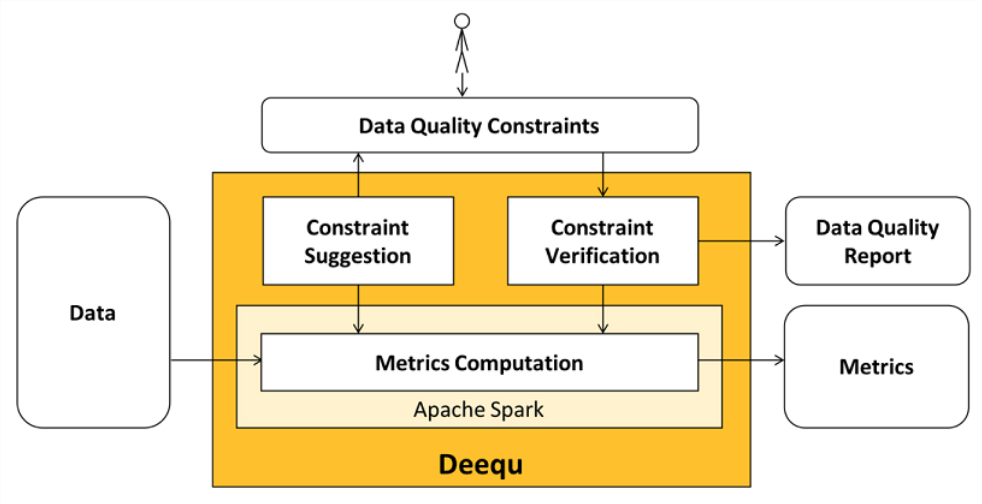
\includegraphics[scale=.4]{deeaqu}
	\caption{Overview of Deequ components.}
	\label{fig:deeaqu}
\end{figure}

\section{Conclusions}

This research paper proposes the NettoyageML that works the impact of data cleaning on ML that regarding to discussed that data quality dimensions through the paper. 

We also observed that only machine learning approaches does not enough to increase quality of data. To increases accuracy of machine learning models of data, we should implement the 
data quality dimensions with real-time verification tools and framework like Amazon's Deequ framework. 
Particularly by using this approaches that help us to reduce junk and mislabeled data sizes on our databases.

We list some research directions; 

\begin{enumerate}
	\item  {Extending the NettoyageML Benchmark, while it represents the most comprehensive work on the subject to date, there are many 
		interesting future extensions. For example we need more datasets with diverse error distributions, especially for the missing values and outliers as the current NettoyageML has no ground truth 
		for these error types.
	}

	\item {
		Identifying the Biases Introduced in Data Cleaning. As discussed, cleaning does not necessarily 
		help and can sometimes  even harm model performance. To decided  whether a given cleaning method should be applied to an ML task.
		We need to detect whether the cleaning process introduce more biases than the dirtiness itself, that is an interesting research point for next researcher.
	}

	\item {
		Holistic cleaning for NettoyageML currently considers each error type that is described separately 
		as a first step to understand how cleaning effects ML. Real-world datasets often exhibit multiple 
		error types and they interact in non-t rival ways.
		Whether the benefits of cleaning are sub-linear, compositional, or super-liner remains an open question.
	}
\end{enumerate}
